%!TEX root = ../../thesis.tex
\chapter{A SSHG Spectroscopic Study of Two Si Surfaces}\label{chap:results}
\partialtoc

In this chapter, I will present the results for the calculation of the nonlinear
susceptibility, $\boldsymbol{\chi}_{\mathrm{surface}}$, and the SSHG yield,
$\mathcal{R}_{\mathrm{iF}}$, for the Si(001)(2$\times$1) and the
Si(111)(1$\times$1):H surfaces. These results are the direct product of all the
theory derived in Chapters \ref{chap:chi2} and \ref{chap:sshgyield}. These
example surfaces provide the perfect testbed for the theory developed in this
work, and the resulting spectra yield insight into the various key aspects of
the theory.

The first part focuses on using the Si(001)(2$\times$1) surface to review and
compare the enhancements that we have added to the framework for calculating
$\boldsymbol{\chi}$. This surface is presented in a special configuration that
allows us to test each improvement made on the theory; namely, the use of the
cut function for extracting the surface susceptibility, the effect of the
scissors operator, and the addition of $\mathbf{v}^{\mathrm{nl}}$. I will also
present a very brief overview of the calculated SSHG yield, but with no
comparison to experimental data as there is very little available for this
surface.

The second part features the Si(111)(1$\times$1):H, which is experimentally
well-characterized, and thus provides an excellent platform with which to test
our robust formulation for the SSHG yield. We will first compare the calculated
$\chi^{xxx}$ component with experimental data from Ref. \cite{hoferAPA96}. This
will provide a nice confirmation of everything we learned from the
Si(001)(2$\times$1) surface. We will then review the calculated spectra for
different polarization cases of the incoming fields, and compare them to
experimental data from Refs. \cite{bergfeldPRL04, mejiaPRB02, mitchellSS01},
over a wide energy range covering both the E$_{1}$ and E$_{2}$ critical point
transitions for bulk Si. We will find that this new formalism, that is developed
from the 3-layer model and includes the effect of multiple reflections in the
material, compares quite favorably with the experimental data. The quality of
these calculations affords us some insight into how the SSHG spectrum can
affected by several physical factors.


%%%%%%%%%%%%%%%%%%%%%%%%%%%%%%%%%%%%%%%%%%%%%%%%%%%%%%%%%%%%%%%%%%%%%%%%%%%%%%%%
%%%%%%%%%%%%%%%%%%%%%%%%%%%%%%%%%%%%%%%%%%%%%%%%%%%%%%%%%%%%%%%%%%%%%%%%%%%%%%%%

\section{Results for the \texorpdfstring{Si(001)(2$\times$1)}{Si(001)(2x1)}
Surface}\label{sec:Si2x1results}

In this section, let us review the characteristics of the Si(001)(2$\times$1)
surface we will be using for the subsequent calculations. This surface provides
an excellent test case to check the consistency of our approach for calculating
$\boldsymbol{\chi}$ with the new elements described in Chap. \ref{chap:chi2}.
For this, I have selected a clean Si(001) surface with a 2$\times$1 surface
reconstruction. The slab for such a surface could be made centrosymmetric by
creating the front and back surfaces with the same 2$\times$1 reconstruction.
However, this particular slab has the lower surface terminated with hydrogen,
producing a terminated, ``ideal'' bulk Si surface. The H atoms saturate the
dangling bonds of the bulk-like Si atoms at the surface, as seen in Fig.
\ref{fig:2x1struc}. Consider the $z$ coordinate pointing out of the surface with
the $x$ coordinate along the crystallographic [011] direction, parallel to the
dimers.

\begin{figure}[t]
\centering
\subbottom[Front view.\label{fig:2x1front}]%
{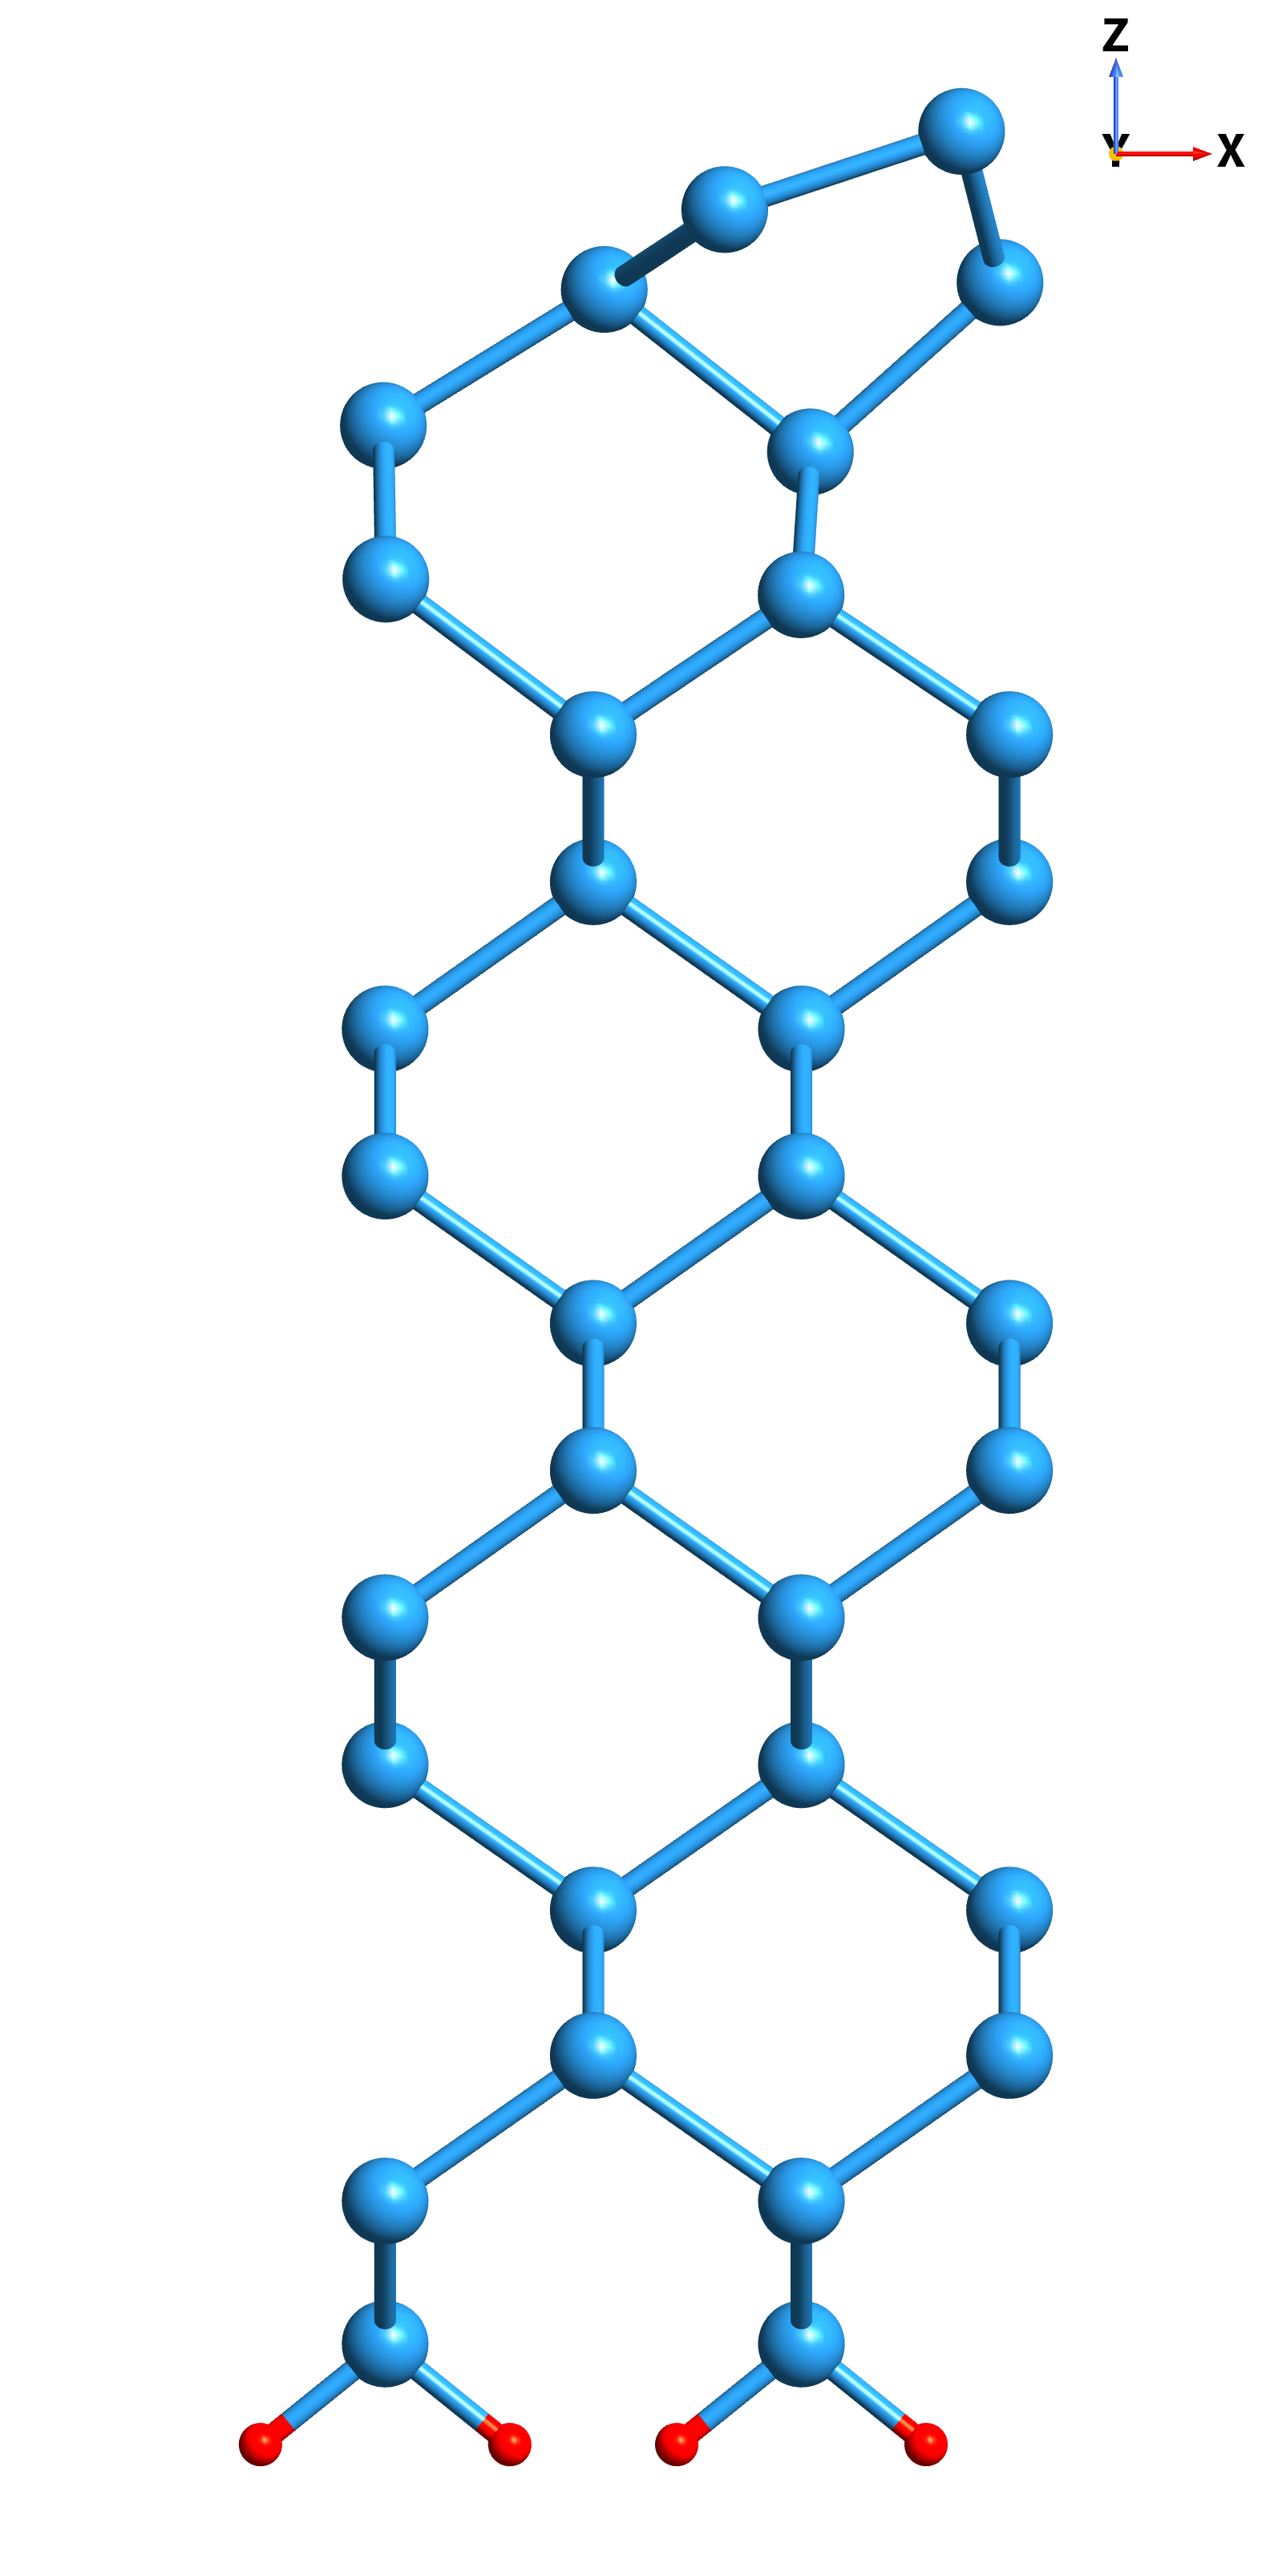
\includegraphics[width=0.3\textwidth]{content/figures/struc-Si2x1-front}}\hfill
\subbottom[Side view.\label{fig:2x1side}]%
{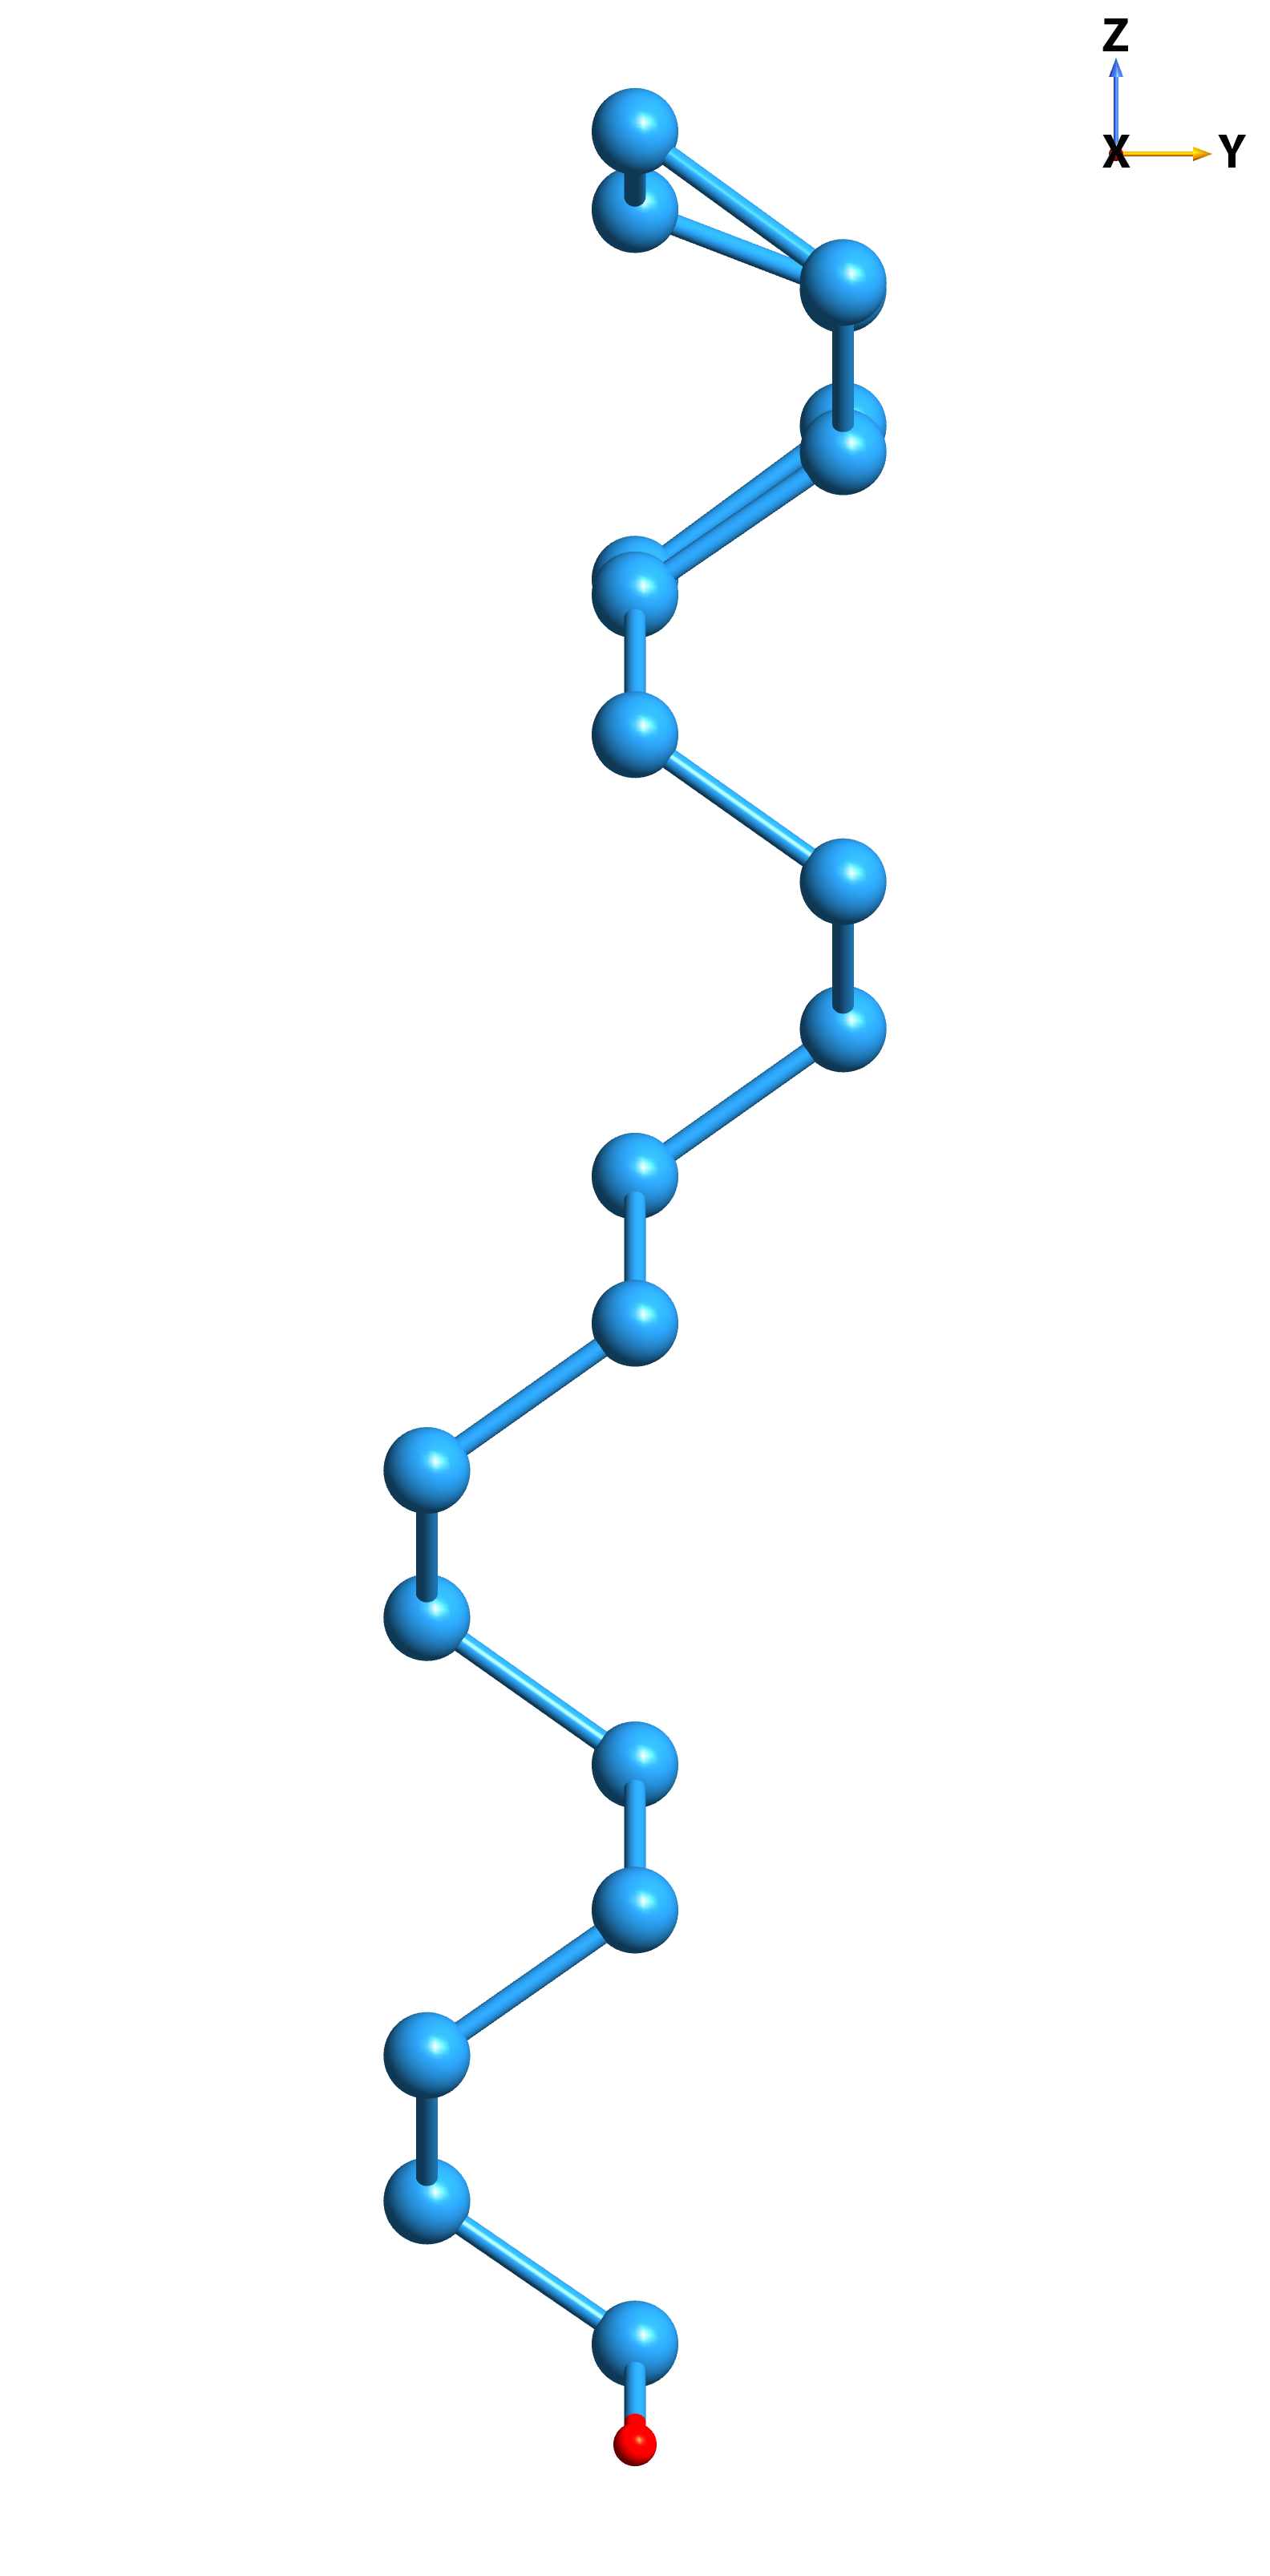
\includegraphics[width=0.3\textwidth]{content/figures/struc-Si2x1-side}}\hfill
\subbottom[Top view.\label{fig:2x1top}]%
{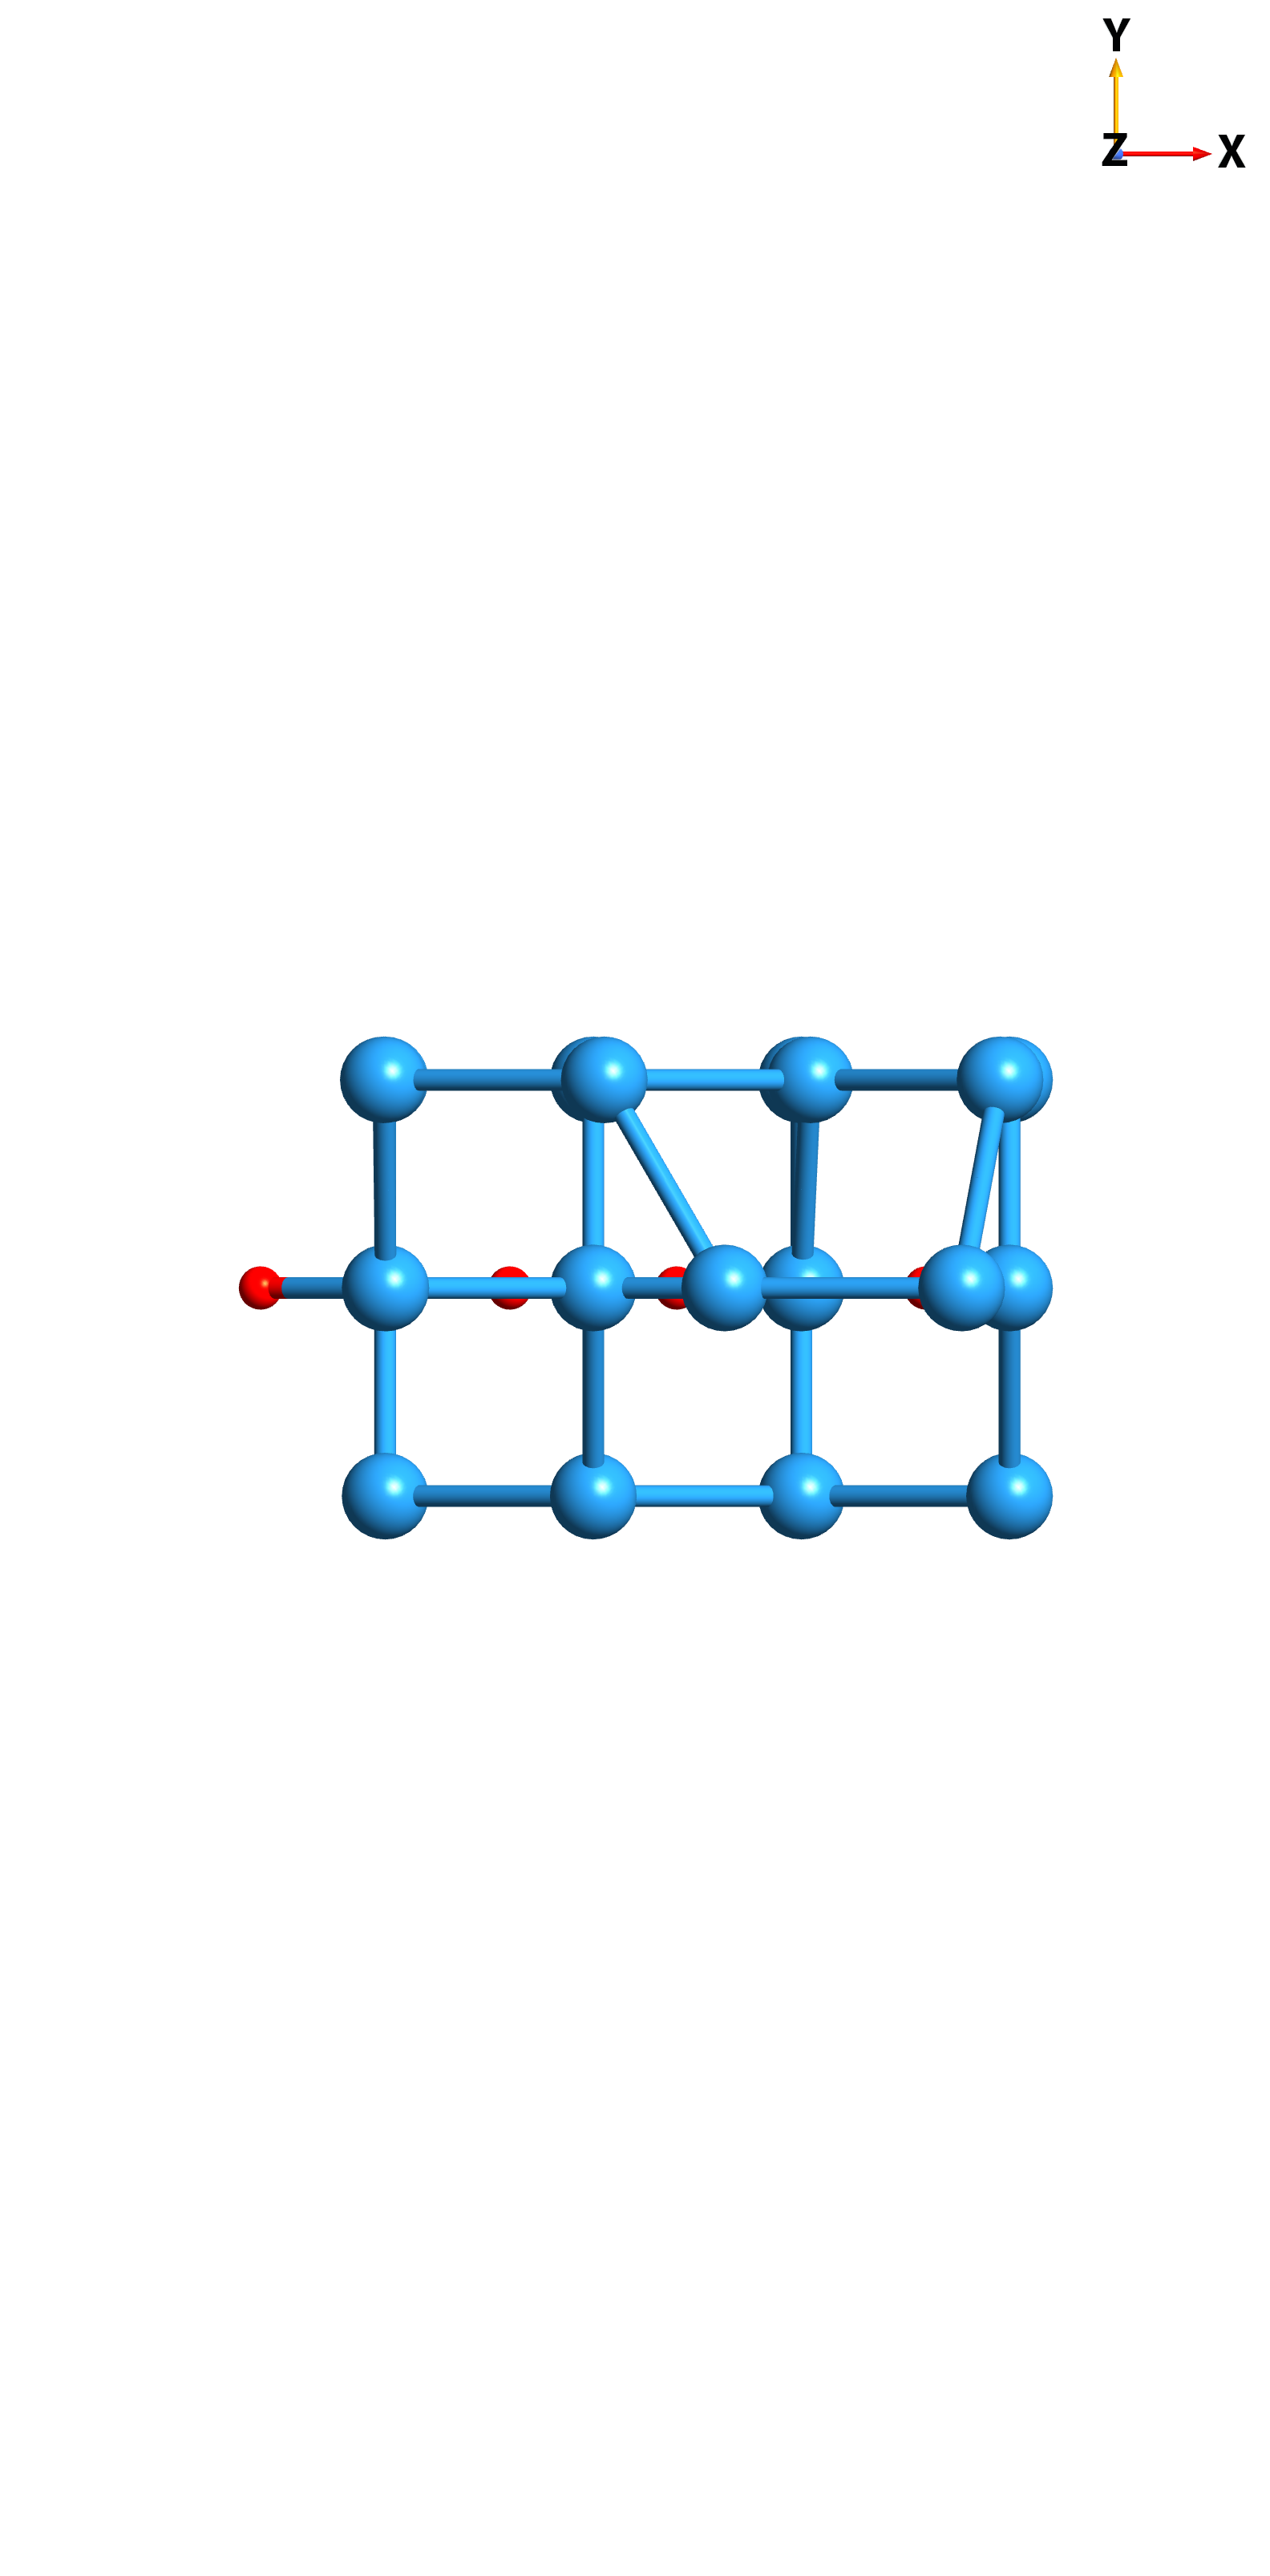
\includegraphics[width=0.3\textwidth]{content/figures/struc-Si2x1-top}}
\caption[Several views of the slab used to represent the Si(001)(2$\times$1)
surface.]
{Several views of the slab used to represent the Si(001)(2$\times$1)
surface. This particular slab has 16 Si atomic layers (large blue balls) with
two H atomic layers (small red balls).}
\label{fig:2x1struc}
\end{figure}

The self-consistent ground state and the Kohn-Sham states were calculated in the
DFT-LDA framework using the plane-wave ABINIT code \cite{gonzeCPS09, abinit},
using Troullier-Martins pseudopotentials \cite{troullierPRB91} that are fully
separable nonlocal pseudopotentials in the Kleinman-Bylander form
\cite{kleinmanPRL82}. The contribution of $\mathbf{v}^\mathrm{nl}$ and
$\boldsymbol{\mathcal{V}}^\mathrm{nl}$ to Eq. \eqref{eq:chis} was carried out
using the DP code \cite{olevanoDP}, which is implemented in our in the TINIBA
code \cite{tiniba} developed at the Centro de Investigaciones en \'Optica, A.C.
The surface was studied with the experimental lattice constant of 5.43 \AA.
Structural optimizations were also performed with the ABINIT code. The geometry
optimization was carried out in slabs of 12 atomic layers, where the central
four layers where fixed at the bulk positions. The structures were relaxed until
the Cartesian force components were less than 5 meV/\AA. The geometry
optimization for the clean surface gives a dimer buckling of 0.721 \AA, and a
dimer length of 2.301 \AA. For the dihydride surface, the obtained Si-H bond
distance was 1.48 \AA. These results are in good agreement with previous
theoretical studies \cite{caramellaPRB09, mendozaPRB06}. The vacuum size is
equivalent to one quarter the size of the slab, avoiding the effects produced by
possible wave-function tunneling from the contiguous surfaces of the full
crystal formed by the repeated super-cell scheme \cite{mendozaPRB06}. Note that
all spectra for $\chi^{xxx}$ presented in this section were calculated with a
Gaussian broadening of 0.15 eV.

Spin-orbit, local field, and electron-hole attraction \cite{beyond} effects on
the SHG process are all neglected. Although these are important factors in the
optical response of a semiconductor, their efficient calculation is still
theoretically and numerically challenging and under debate. This merits further
study but is beyond the scope of this thesis. For a given slab size, I found the
converged spectra to obtain the relevant parameters. The most important of these
are: an energy cutoff of 10 Ha for the 16, 24, and 32 layered slabs and 13 Ha
for the 40 layer slab, an equal number of conduction and valence bands, and a
set of 244 \textbf{k} points in the irreducible Brillouin zone, which are
equivalent to 1058 \textbf{k} points when disregarding symmetry relations. The
\textbf{k} points are used for the linear analytic tetrahedron method for
evaluating the 3D Brillouin Zone (BZ) integrals, where special care was taken to
examine the double resonances of Eq. \eqref{eq:chis} \cite{nastosPRB05}. Note
that the Brillouin zone for the slab geometry collapses to a 2D-zone, with only
one $\mathbf{k}$-point along the $z$-axis.


%%%%%%%%%%%%%%%%%%%%%%%%%%%%%%%%%%%%%%%%%%%%%%%%%%%%%%%%%%%%%%%%%%%%%%%%%%%%%%%%

\subsection{Calculating 
\texorpdfstring{$\chi^{xxx}_{\mathrm{surface}}(-2\omega;\omega,\omega)$}{Xxxx}}
\label{sec:res2x1chi}

The idea behind the special slab configuration, pictured in Fig.
\ref{fig:si2x1slab}, is that the crystalline symmetry of the H terminated
surface imposes that $\chi_{\mathrm{H}}^{xxx}=0$. The 2$\times$1 surface has no
such restrictions, so naturally $\chi_{2\times 1}^{xxx}\ne 0$. This is due to
the fact that along the $y$ direction there is a mirror plane for the
H-saturated surface (causing centrosymmetry), whereas for the 2$\times$1 surface
this mirror is lost as the dimers are asymmetric along $x$. Thus, calculating
$\chi^{xxx}$ for the full-slab, or the upper half-slab containing the 2$\times$1
surface \cite{note1} should yield the same result, since the contribution from
the H saturated surface is zero either way. The following relationship must be
satisfied for this particular slab,
\begin{equation*}
\chi_{\mathrm{half-slab}}^{xxx} =
\chi_{\mathrm{full-slab}}^{xxx},
\end{equation*}
where $\chi_{\mathrm{half-slab}}^{xxx}$ is calculated using
${\mathbf{\mathcal{C}}}(z) = 1$ for the upper half containing the 2$\times$1
surface reconstruction (see Fig. \ref{fig:si2x1slab}), and
$\chi_{\mathrm{full-slab}}^{xxx}$ is calculated using ${\mathbf{\mathcal{C}}}(z)
= 1$ for the entire slab. Again, the dihydride surface on the lower half of the
slab must have $\chi_{\mathrm{half-slab}}^{xxx} = 0$.

\begin{figure}[h]
\centering 
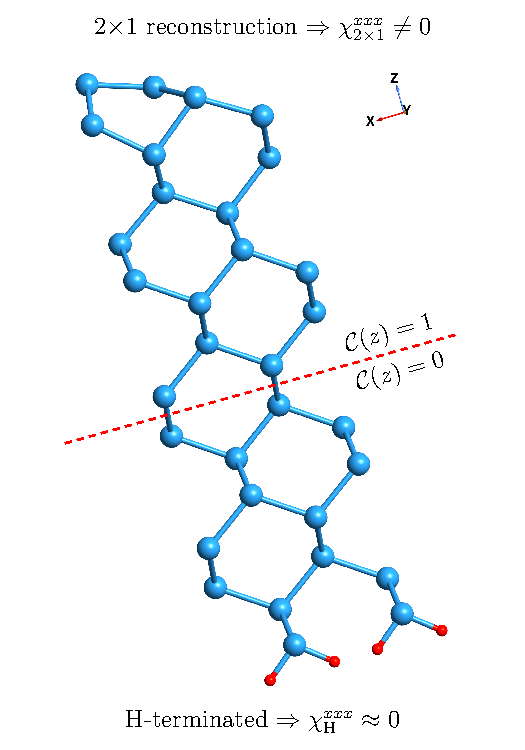
\includegraphics[width=0.4\textwidth]{content/figures/struc-Si2x1-rot}
\caption[The slab for the Si(001)(2$\times$1) surface.]
{The slab for the Si(001)(2$\times$1) surface. The front (upper) surface
is in a 2$\times$1, clean reconstruction, and the rear (lower) surfaces is
H-terminated, with ``ideal'' bulk-like atomic positions. The dangling bonds are
H-saturated.}
\label{fig:si2x1slab}
\end{figure} 


%%%%%%%%%%%%%%%%%%%%%%%%%%%%%%%%%%%%%%%%%%%%%%%%%%%%%%%%%%%%%%%%%%%%%%%%%%%%%%%%

\subsubsection{Full-slab Results}\label{sec:fsresults}

Fig. \ref{fig:layersconv} shows $|\chi_{\mathrm{full-slab}}^{xxx}|$ for the slab
with 16, 24, 32, and 40 Si atomic layers, without the contribution of
$\mathbf{v}^{\mathrm{nl}}$, and with no scissors correction. Since the clean
Si(001) surface is in a 2$\times$1 reconstruction there are two atoms per atomic
layer. Thus, the total number of atoms per slab is twice the number of atomic
layers of the slab. The slabs were extended in the $z$ directions in steps of 8
layers of bulk-like atomic positions. Note that the response differs
substantially for 16 and 24 layers but is quite similar for 32 and 40 layers. As
explained above, the calculation of the $\mathbf{v}^\mathrm{nl}$ contribution is
computationally expensive, so it is crucial to minimize the number of atoms in
the calculation. I consider a slab with 32 Si atomic layers as a good compromise
between the convergence of $\chi^{xxx}_{\mathrm{full-slab}}$ as a function of
the number of layers in the slab, and the computational expense.

\begin{figure}[H]
\centering 
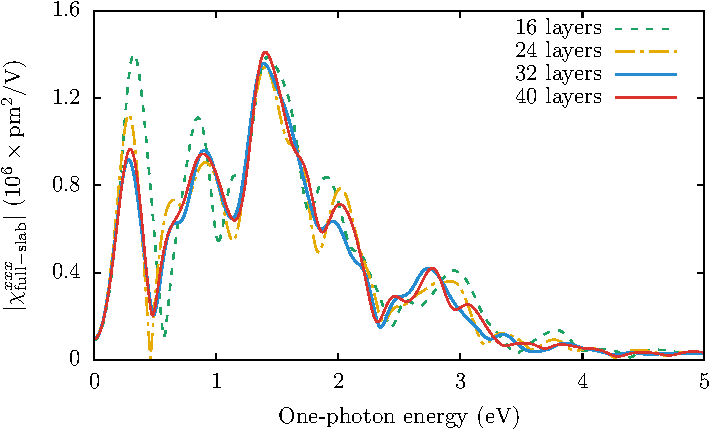
\includegraphics[width=0.6\textwidth]{content/figures/fig-Si2x1-layerconv}
\caption[Layer convergence for the Si(001)(2$\times$1) slab.]
{$\vert\chi_{\mathrm{full-slab}}^{xxx}\vert$ vs $\hbar\omega$ for the
slab with 16, 24, 32, and 40 atomic Si layers. Adequate convergence is achieved
after 32 layers. The spectra presented here use a scissors value of $\hbar\Delta
= 0$ eV, and do not include the contribution from $\mathbf{v}^{\mathrm{nl}}$.}
\label{fig:layersconv}
\end{figure}


%%%%%%%%%%%%%%%%%%%%%%%%%%%%%%%%%%%%%%%%%%%%%%%%%%%%%%%%%%%%%%%%%%%%%%%%%%%%%%%%

\subsubsection{Half-slab vs Full-slab}

Now that we have established an adequate number of layers to attain convergence,
we can proceed to study the spectra produced from the slab with 32 atomic
layers. Fig. \ref{fig:hsvfs} presents a comparison between
$\chi^{xxx}_{\mathrm{half-slab}}$ and $\chi^{xxx}_{\mathrm{full-slab}}$ for four
different scenarios: with and without the effects of $\mathbf{v}^\mathrm{nl}$,
and with two values for the scissors correction, $\hbar\Delta$. I have chosen a
scissors value of $\hbar\Delta=0.5$ eV, that is the GW gap reported in Refs.
\cite{rohlfingPRB95, garciaCPC01}. This is justified by the fact that the
surface states from the clean 2$\times$1 surface are rigidly shifted and
maintain their dispersion relation with respect to the LDA value, according to
the GW calculations of Ref.
\cite{rohlfingPRB95}.

We can appreciate that the difference between the half-slab and full-slab
responses is quite small for all four scenarios. Indeed, when the value
$\vert\chi^{xxx}\vert$ is large, the difference between the two is quite small;
when $\vert\chi^{xxx}\vert$ is small, the difference increases slightly but the
spectra is so close to zero that it is negligible. Of course, the difference
between the two would decrease as the number of atomic layers increases. Note
how 32 layers in the slab is more than enough to confirm that the extraction of
the surface second-harmonic susceptibility from the 2$\times$1 surface is
readily possible using the formalism contained in Eq. \eqref{eq:chis}.
Calculating the response from the lower half of the slab substantiates that
$\vert\chi^{xxx}_{\mathrm{half-slab}}\vert\approx 0$ for the dihydride surface,
shown in Fig. \ref{fig:topvbottom}.

\begin{figure}[H]
\centering 
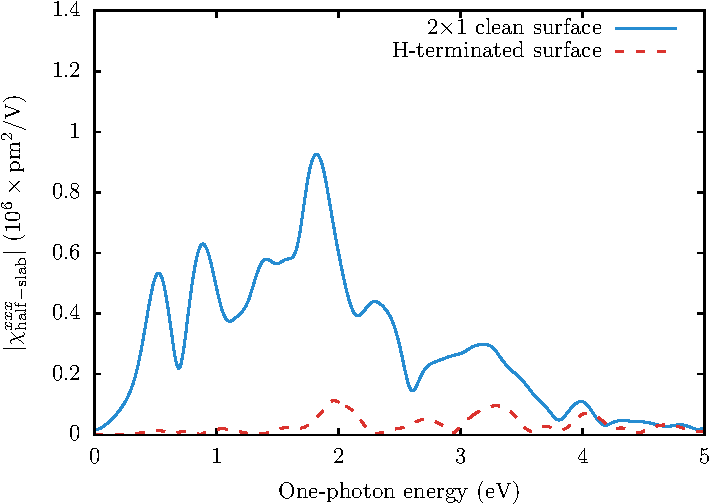
\includegraphics[width=0.6\textwidth]{content/figures/fig-Si2x1-topvbottom}
\caption[$\chi^{xxx}_{\mathrm{half-slab}}$ for the clean and H-terminated 
surfaces.]
{$\chi^{xxx}_{\mathrm{half-slab}}$ vs $\hbar\omega$ for the clean
2$\times$1 and H-terminated surfaces, with $\hbar\Delta = 0.5$ eV and without
the effects of $\mathbf{v}^\mathrm{nl}$.}
\label{fig:topvbottom}
\end{figure}

This confirms the validity of the theory developed in Chapter \ref{chap:chi2}
and is an important result of this work. Through the proposed layer formalism,
we can calculate the surface $\chi^{\mathrm{abc}}$ component including the
contribution from the nonlocal part of the pseudopotentials, and part of the
many-body effects through the scissors correction. Therefore, this scheme is
robust and versatile and should work for any crystalline surface.

\clearpage
\begin{figure}[H]
\centering 
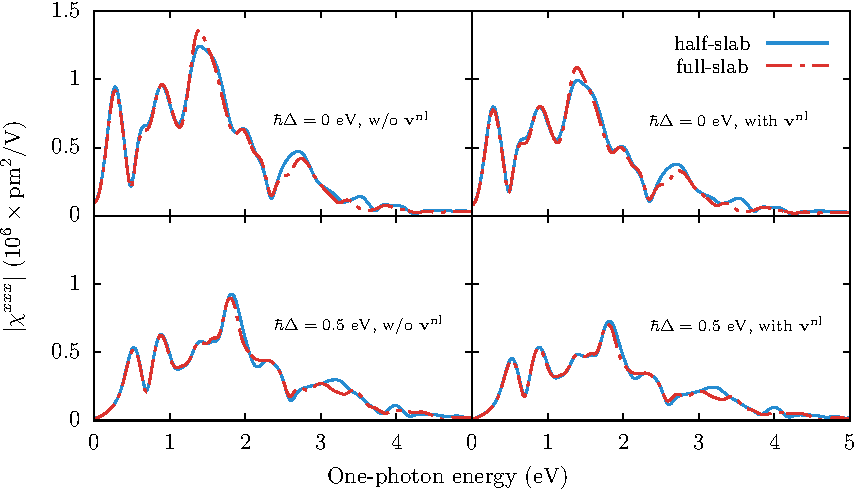
\includegraphics[height=0.9\textheight]{content/figures/fig-Si2x1-hsvsfs}
\caption[Different scenarios of half-slab vs full-slab.]
{$\chi^{xxx}_{\mathrm{half-slab}}$ and $\chi^{xxx}_{\mathrm{full-slab}}$
vs $\hbar\omega$ for four different combinations: with and without the effects
of $\mathbf{v}^\mathrm{nl}$, and with two values for the scissors correction,
$\hbar\Delta$.}
\label{fig:hsvfs}
\end{figure}


%%%%%%%%%%%%%%%%%%%%%%%%%%%%%%%%%%%%%%%%%%%%%%%%%%%%%%%%%%%%%%%%%%%%%%%%%%%%%%%%

\subsubsection{Half-slab Results}

I proceed to explain some of the features seen in
$\vert\chi^{xxx}_{\mathrm{half-slab}}\vert$ that is obtained when setting
$\mathbf{\mathcal{C}}(z) = 1$ for the upper half containing the 2$\times$1
surface reconstruction, as seen in Fig. \ref{fig:si2x1slab}. From Fig.
\ref{fig:hsvfs}, we note a series of resonances that derive from the $1\omega$
and $2\omega$ terms in Eq. \eqref{eq:chis}. Notice that the $2\omega$ resonances
start below $E_{g}/2$, where $E_{g}$ is the band gap (0.53 eV for LDA, and 1.03
eV if the scissor is used with $\hbar\Delta=0.5$ eV). These resonances come from
the electronic states of the 2$\times$1 surface, that lie inside the bulk band
gap of Si and are the well known electronic surface states \cite{rohlfingPRB95}.

Fig. \ref{fig:vnl} shows that the inclusion of $\mathbf{v}^\mathrm{nl}$ reduces
the value of $\vert\chi^{xxx}_{\mathrm{half-slab}}\vert$ by 15-20\%. This
demonstrates the importance of this contribution for a fully correct SSHG
calculation. This is in agreement with the analysis for bulk semiconductors
\cite{luppiPRB08}. However, the inclusion of $\mathbf{v}^\mathrm{nl}$ does not
change the spectral shape of $\vert\chi^{xxx}_{\mathrm{half-slab}}\vert$. We can
confirm that this is not unique for this specific scissors shift, as we can
appreciate from the upper two panels of Fig. \ref{fig:hsvfs}, with $\hbar\Delta
= 0$ eV.

\begin{figure}[b]
\centering 
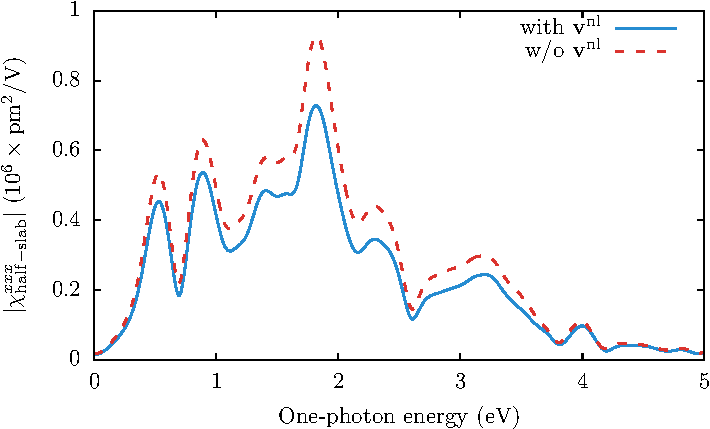
\includegraphics[width=0.6\textwidth]{content/figures/fig-Si2x1-vnl}
\caption[$\chi^{xxx}_{\mathrm{half-slab}}$ with and without
$\mathbf{v}^\mathrm{nl}$]
{$\chi^{xxx}_{\mathrm{half-slab}}$ vs $\hbar\omega$, with and without
the contribution from $\mathbf{v}^\mathrm{nl}$. This spectrum has a scissors
value of $\hbar\Delta=0.5$ eV.}
\label{fig:vnl}
\end{figure}

To demonstrate the effect of the scissors correction, I considered two different
finite values for $\hbar\Delta$. The first, with a value of $\hbar\Delta=0.5$ eV
that is used in the previous results, is the ``average'' GW gap taken from Ref.
\cite{rohlfingPRB95} that is in agreement with Ref. \cite{garciaCPC01}. The
second, with a value of $\hbar\Delta=0.63$ eV is the ``average'' gap taken from
Ref. \cite{asahiPRB00}, where more \textbf{k} points in the Brillouin zone were
used to calculate the GW value. Fig. \ref{fig:scissors} shows that the scissors
correction shifts the spectra from its LDA value to higher energies, as
expected. However, contrary to the case of linear optics \cite{cabellosPRB09},
the shift introduced by the scissors correction is not rigid, which is
consistent with the work of Ref. \cite{nastosPRB05}. This is because the
second-harmonic optical response mixes $1\omega$ and $2\omega$ transitions (see
Eq. \eqref{eq:chis}), and accounts for the non-rigid shift. The reduction of the
spectral strength is in agreement with previous calculations for bulk systems
\cite{nastosPRB05, luppiPRB10, leitsmannPRB05}. When comparing
$\vert\chi^{xxx}_{\mathrm{half-slab}}\vert$ for the two finite values of
$\hbar\Delta$, it is clear that the first two peaks are almost rigidly shifted
with a small difference in height while the rest of the peaks are modified
substantially. This behavior comes from the fact that the first two peaks are
almost exclusively related to the $2\omega$ resonances of Eq.
\eqref{eq:chis}. The other peaks are a combination of $1\omega$ and $2\omega$
resonances and yield a more varied spectrum. Note that for large-gap materials
the $1\omega$ and $2\omega$ resonances would be split, producing a small
interference effect. The $2\omega$ resonances would still strongly depend on the
surface states. Thus, small changes in the scissors shift can affect the SSH
susceptibility spectrum quite dramatically. In Ref. \cite{adolphPRB00}, the
authors already noted that the nonlinear optical response of bulk materials is
more influenced by the electronic structure of the material than the linear
case. For the case of semiconductor surfaces, the problem is even more intricate
due to the presence of electronic surface states.

\begin{figure}[b]
\centering 
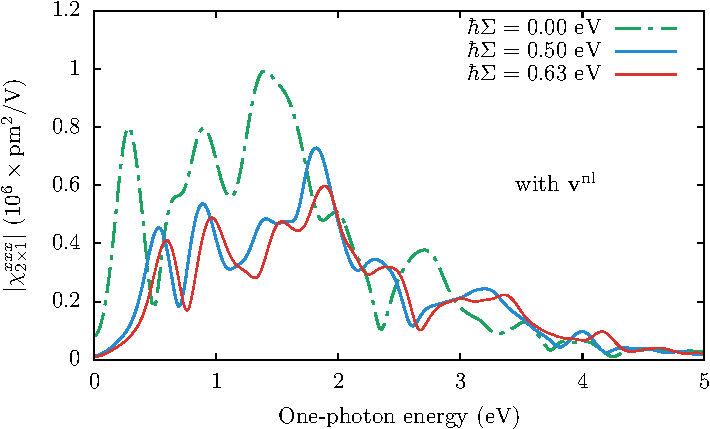
\includegraphics[width=0.6\textwidth]{content/figures/fig-Si2x1-scissors}
\caption[$\chi^{xxx}_{\mathrm{half-slab}}$ with three different values of the 
scissors correction.]
{$\chi^{xxx}_{\mathrm{half-slab}}$ vs $\hbar\omega$ for a slab with 32
atomic Si layers plus one H layer, for three different values of the scissors
correction, $\hbar\Delta$.
\label{fig:scissors}} 
\end{figure}

The high sensitivity of SSHG to the energy position of surface states, as seen
in Fig. \ref{fig:scissors}, makes SSHG a good benchmark tool for
spectroscopically testing the validity of the inclusion of many-body effects,
and in particular the quasi-particle correction to the electronic states.
Although local fields are neglected, in principle they should be quite small
parallel to the interface as the electric field is continuous. $\chi^{xxx}$
should have a relatively small influence from these local fields. Excitonic
effects should also be explored, but their efficient calculation is
theoretically and numerically challenging \cite{beyond} and far beyond the scope
of this work. Unfortunately the experimental measurement of the $\chi^{xxx}$
component is difficult as the SH radiated intensity would be proportional not
only to this component but also to the other components of $\boldsymbol{\chi}$.
However, I will present this comparison later on in Sec. \ref{sec:res1x1chi} for
the Si(111)(1$\times$1):H surface.


%%%%%%%%%%%%%%%%%%%%%%%%%%%%%%%%%%%%%%%%%%%%%%%%%%%%%%%%%%%%%%%%%%%%%%%%%%%%%%%%

\subsection{Overview of the Calculated \texorpdfstring{$\mathcal{R}$}{R}
Spectra}\label{sec:2x1R3D}

In Figs. \ref{fig:2x1rP3d} and \ref{fig:2x1rS3d}, I present the results for the
calculation of the SSHG yield for our test surface. The 2$\times$1 surface
reconstruction yields a Class 1, primitive triclinic system with all 18
components independent from each other \cite{popovbook}. We cannot take
advantage of any symmetry relations for this surface. However, this is no
problem for the robust formulation we derived in Chapter \ref{chap:sshgyield}
that can accommodate all 18 components disregarding any surface symmetries.
Calculating all 18 components is obviously more time consuming, but this
calculation can be parallelized in order to calculate all components at once, so
very little time is actually lost.

\begin{figure}[b]
\centering
\subbottom[$\mathcal{R}_{pP}$\label{fig:2x1rpp3d}]%
{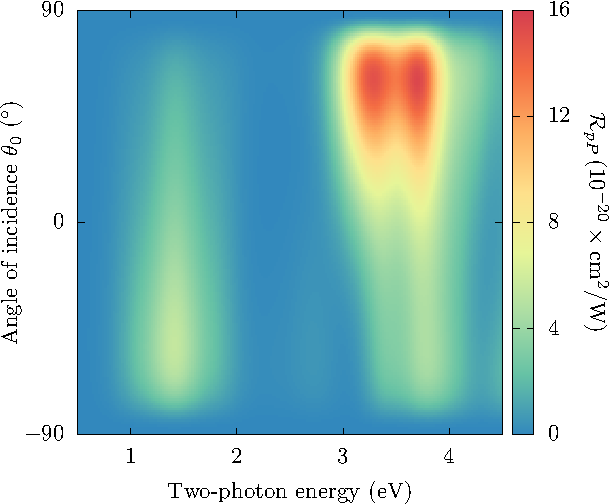
\includegraphics[height=0.4\textwidth]{content/figures/3D-Si2x1-RpP.pdf}}\hfill
\subbottom[$\mathcal{R}_{sP}$\label{fig:2x1rsp3d}]%
{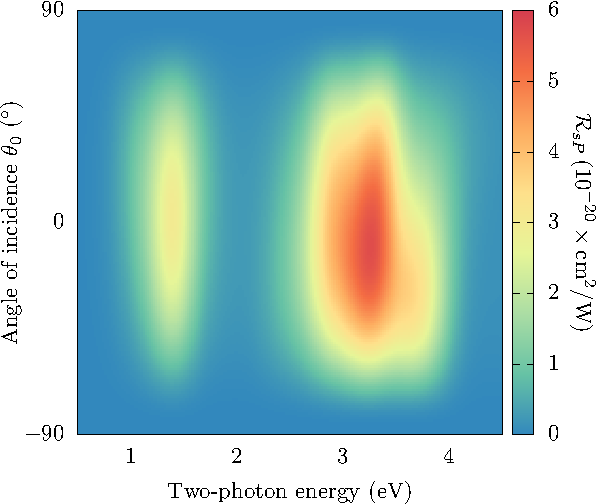
\includegraphics[height=0.4\textwidth]{content/figures/3D-Si2x1-RsP.pdf}}
\caption[Overview of the angular dependence of $\mathcal{R}_{\mathrm{iP}}$.]
{$\mathcal{R}$ for outgoing $P$ polarization, versus the angle of
incidence ($\theta_{0}$) for the Si(001)(2$\times$1) surface. The scissor shift
used was $\hbar\Delta = 0.5$ eV. Both figures consider an azimuthal angle of
$\phi = 45^{\circ}$.}
\label{fig:2x1rP3d}
\end{figure}

Fig. \ref{fig:2x1rP3d} presents the results for the SSHG yield with outgoing $P$
polarization. I set a fixed azimuthal angle of $\phi = 45^{\circ}$ and then
varied the incoming angle $\theta_{0}$ from $-90^{\circ}$ to $90^{\circ}$. We
can clearly see that the surface states associated with the 2$\times$1
reconstruction produce significant intensity between 1-2 eV in the two-photon
energy range. This is consistent with the findings presented in the previous
section and in Ref. \cite{andersonPRB15}. The intensity of the peak related to
the surface states is significantly lower than the peaks produced in the 2.5-4
eV two-photon energy range. The spectrum for $\mathcal{R}_{pP}$ is very
consistent with other calculations of this type
\cite{tancognedejean:tel-01235611}, and even with some limited experimental data
\cite{powerPRL95}.

\begin{figure}[t]
\centering
\subbottom[$\mathcal{R}_{pS}$\label{fig:2x1rps3d}]%
{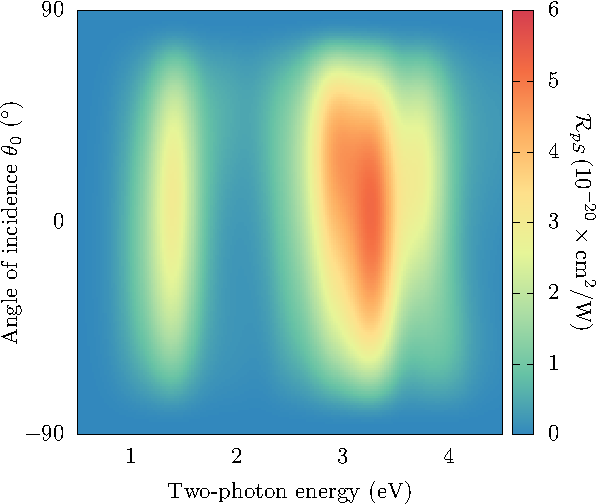
\includegraphics[height=0.4\textwidth]{content/figures/3D-Si2x1-RpS.pdf}}\hfill
\subbottom[$\mathcal{R}_{sS}$\label{fig:2x1rss3d}]%
{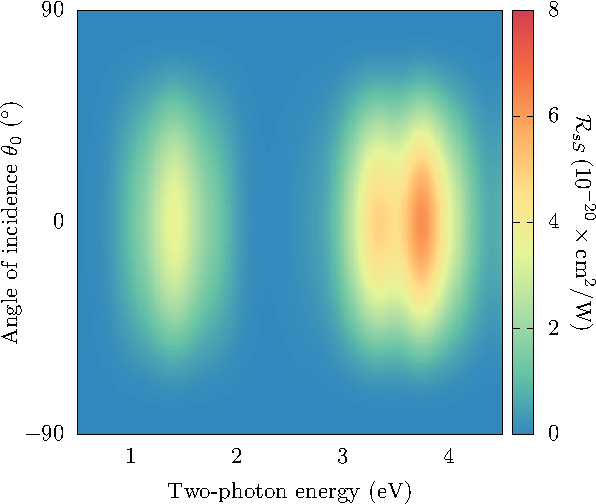
\includegraphics[height=0.4\textwidth]{content/figures/3D-Si2x1-RsS.pdf}}
\caption[Overview of the angular dependence of $\mathcal{R}_{\mathrm{iS}}$.]
{$\mathcal{R}$ for outgoing $S$ polarized fields, versus the angle of
incidence ($\theta_{0}$) for the Si(001)(2$\times$1) surface. The scissor shift
used was $\hbar\Delta = 0.5$ eV. Both figures consider an azimuthal angle of
$\phi = 45^{\circ}$.}
\label{fig:2x1rS3d}
\end{figure}

Fig. \ref{fig:2x1rS3d} presents the results for the SSHG yield with outgoing $S$
polarization. They are quite similar to what we observed in Fig.
\ref{fig:2x1rP3d}, with a peak related to the surface states between 1-2 eV, and
a larger set of peaks between 2.4-4 eV in the two-photon energy range. These
spectra have a clear maxima around $\theta_{0} = 0^{\circ}$. These plots are
presented for mainly illustrative purposes, as there is little experimental data
to compare with the theoretical spectrum. However, these kinds of plots will be
quite useful to the experimentalist interested in this kind of spectroscopy.
Excellent intensity for all polarization cases can be obtained for small beam
angles, such as $\theta_{0} = 30^{\circ}$.


%%%%%%%%%%%%%%%%%%%%%%%%%%%%%%%%%%%%%%%%%%%%%%%%%%%%%%%%%%%%%%%%%%%%%%%%%%%%%%%%
%%%%%%%%%%%%%%%%%%%%%%%%%%%%%%%%%%%%%%%%%%%%%%%%%%%%%%%%%%%%%%%%%%%%%%%%%%%%%%%%

\section{Results for the \texorpdfstring{Si(111)(1$\times$1):H}{Si(111)(1x1):H}
Surface}\label{sec:Si1x1results}

We will now focus our attention on the Si(111)(1$\times$1):H surface. This
surface is a $C_{3v}$, primitive hexagonal system with only 4 nonzero components
independent from each other, as shown in Table \ref{tab:chis} \cite{popovbook,
sipePRB87, mizrahiJOSA88}. It is composed of stacked layers with one Si atom
each, with one H atom terminating each surface. The added H saturates the
surface Si dangling bonds and eliminates any surface-related electronic states
in the band gap. Here, the top and bottom surfaces are mirror images (see Fig.
\ref{fig:1x1struc}); this provides the centrosymmetry that necessitates the use
of the cut function to extract the nonzero surface response. In Sec.
\ref{sec:res1x1chi} we will compare the spectrum produced by using relaxed and
unrelaxed coordinates, so it is worth reviewing this concept here. The specifics
of this process are as follows.

The relaxation process was done by my colleague, Nicolas Tancogne-Dejean
\cite{tancognedejean:tel-01235611}. The structure was initially constructed with
the experimental lattice constant of 5.43 \AA, and then performed structural
optimizations with the ABINIT \cite{gonzeCPS09, abinit} code. It was then
relaxed until the Cartesian force components were less than 5 meV/\AA, yielding
a final Si-H bond distance of 1.50 \AA. The energy cutoff used was 20 Ha, and
Troullier-Martin LDA pseudopotentials were used \cite{troullierPRB91}. The
resulting atomic positions are in good agreement with previous theoretical
studies \cite{kaxirasPRB88, jonaPRB95, alfonsoPRB96, cargnoniJOCP00,
mejiaPRB02}, as well as the experimental value for the Si-H distance
\cite{weastCRC88}.

I also evaluated the number of layers required for convergence (like Sec.
\ref{sec:fsresults}) and settled on a slab with 48 atomic Si planes. The
geometric optimizations mentioned above are therefore carried out on slabs of 48
atomic layers without fixing any atoms to the bulk positions. Fig.
\ref{fig:1x1struc} depicts a sample slab with 16 layers of Si. The surface
susceptibilities must be extracted from only half of the slab. This encompasses
24 layers of Si and the single layer of H that terminates the top surface. The
vacuum size is equivalent to one quarter the size of the slab, avoiding the
effects produced by possible wave-function tunneling from the contiguous
surfaces of the full crystal formed by the repeated super-cell scheme
\cite{mendozaPRB06}.

\begin{figure}[t]
\centering
\subbottom[Front view.\label{fig:1x1front}]%
{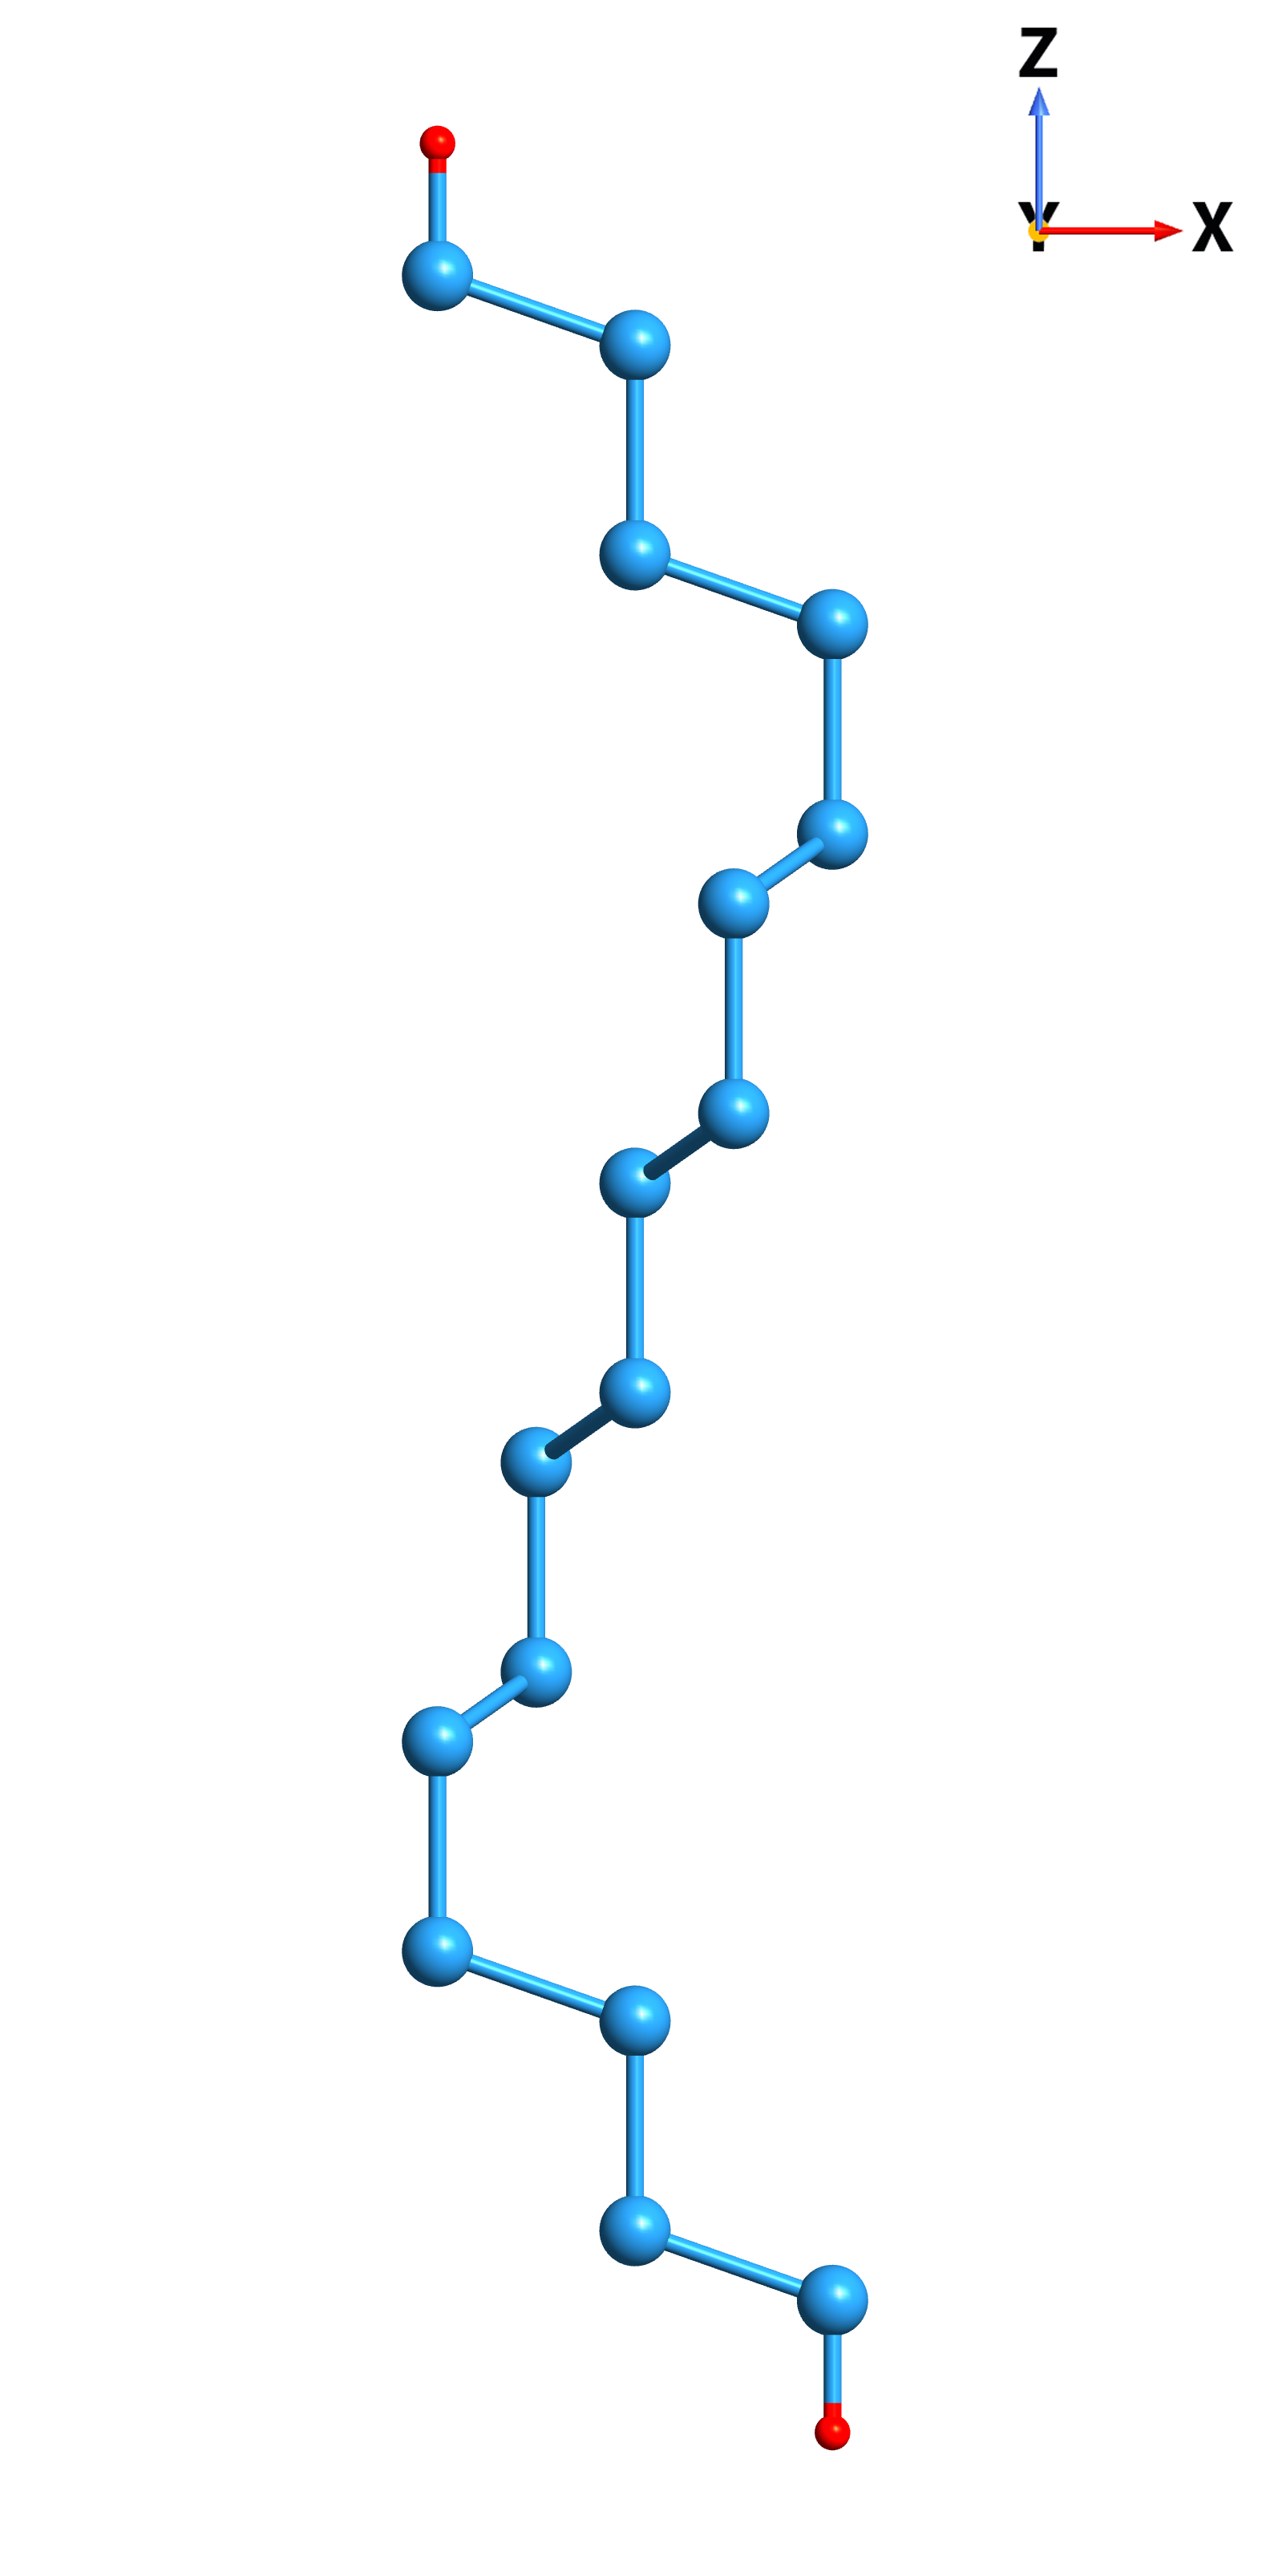
\includegraphics[width=0.3\textwidth]{content/figures/struc-Si1x1-front}}\hfill
\subbottom[Side view.\label{fig:1x1side}]%
{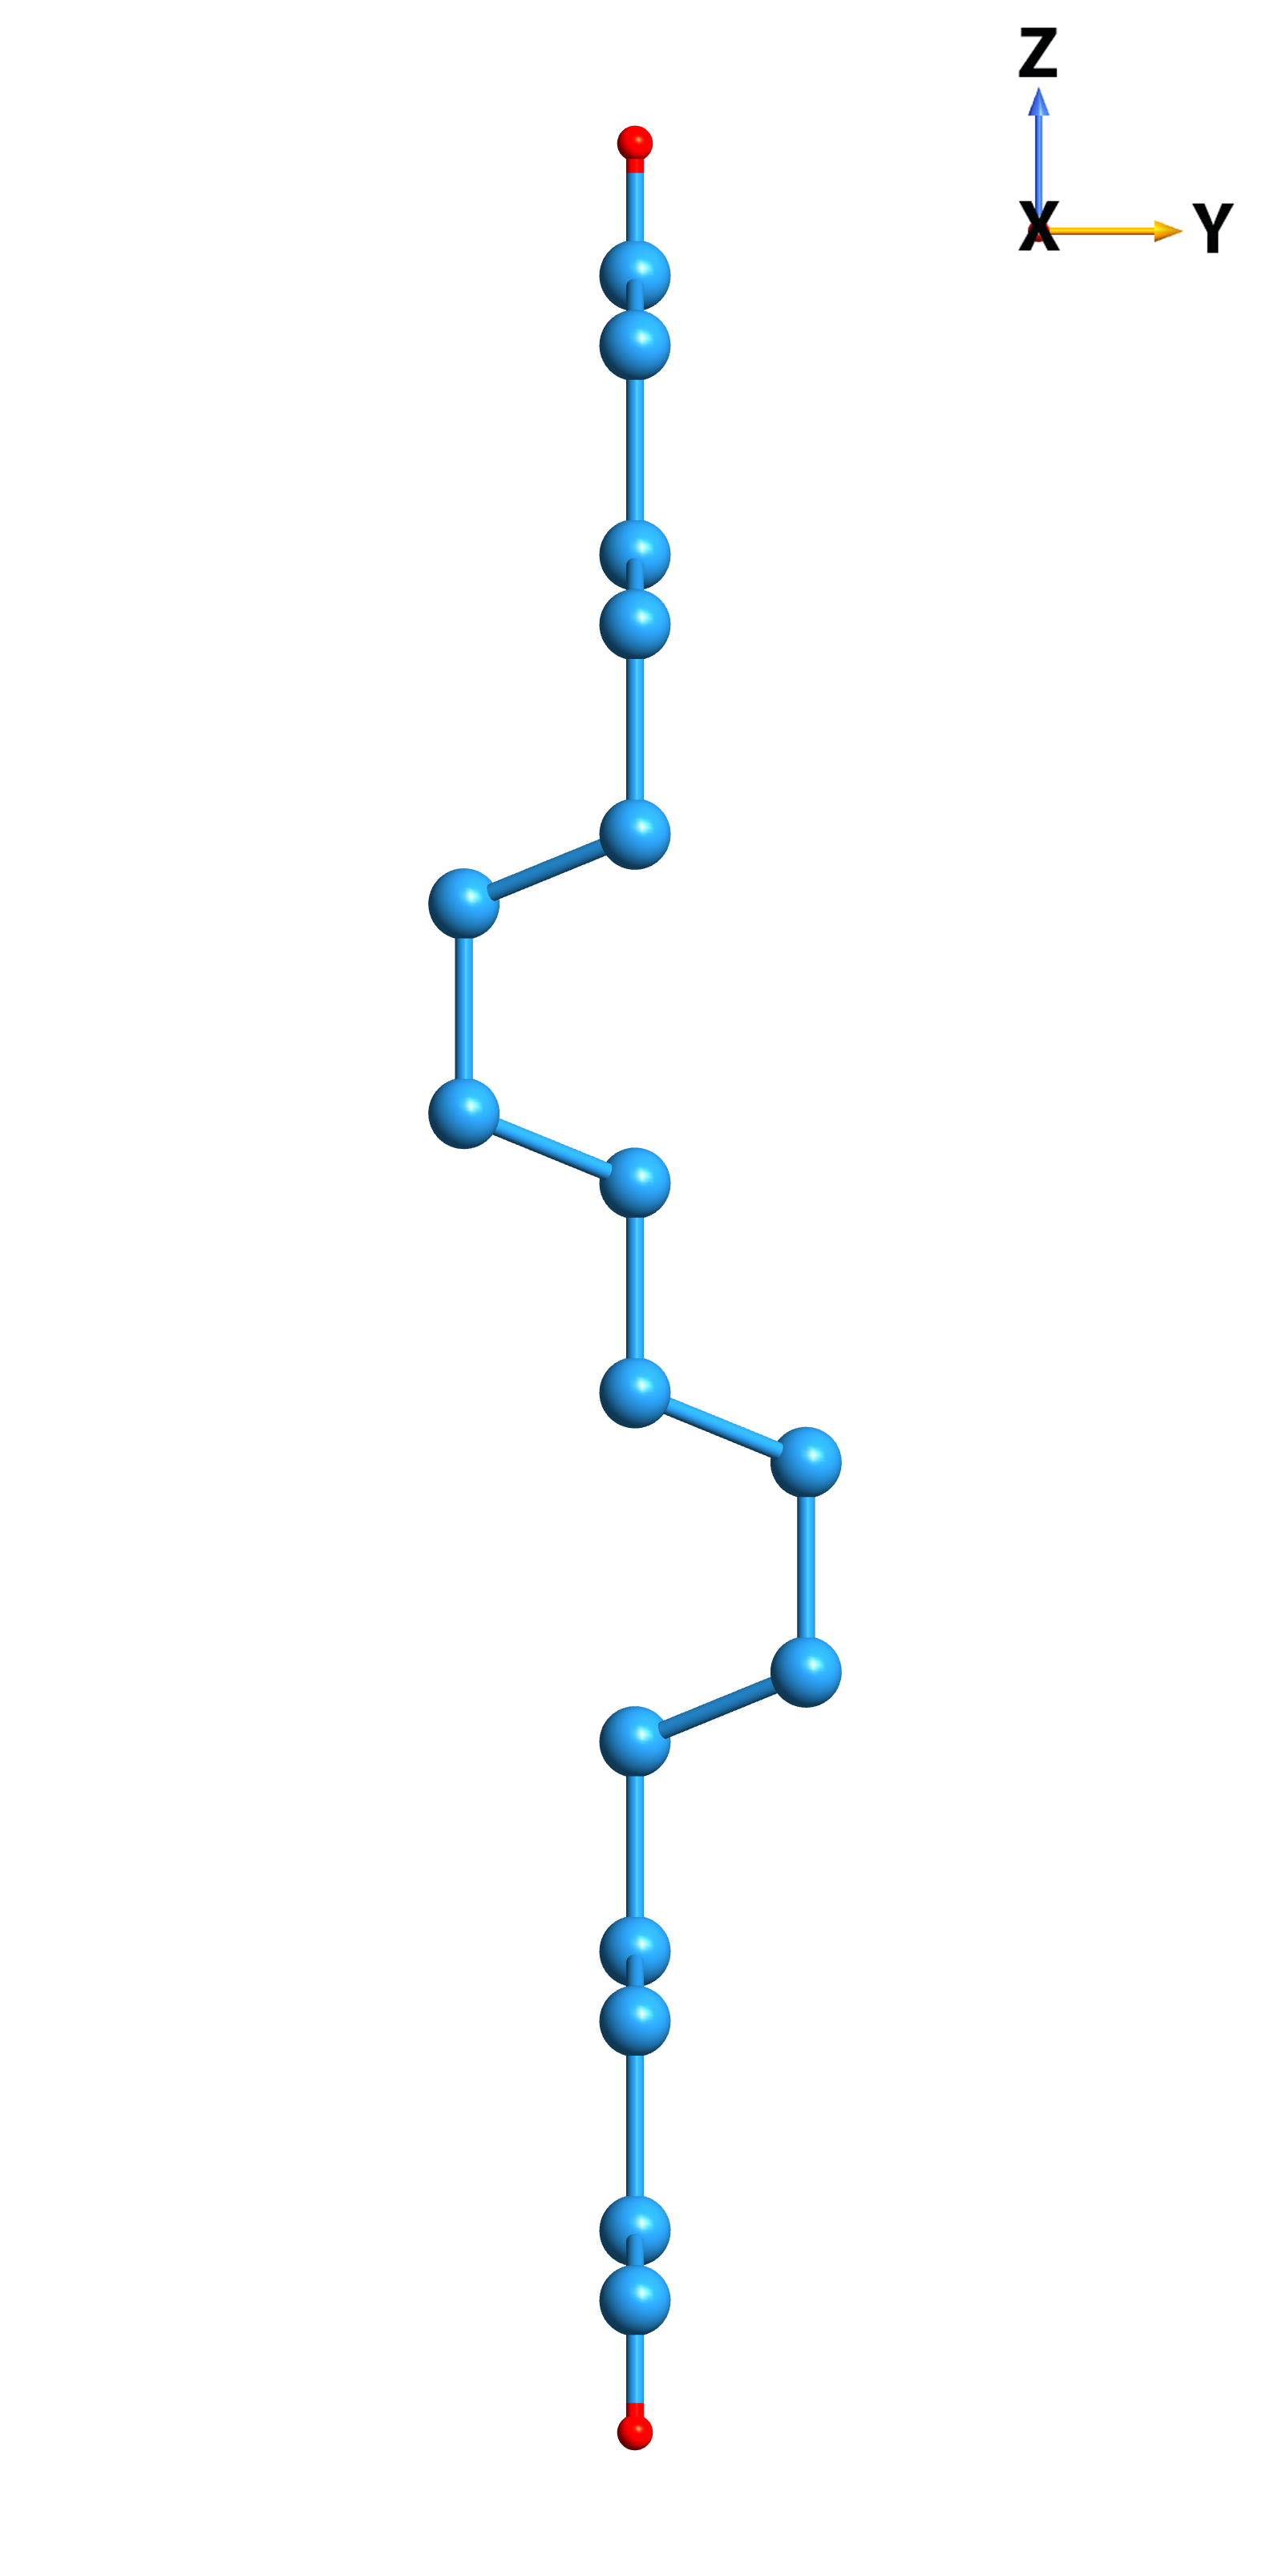
\includegraphics[width=0.3\textwidth]{content/figures/struc-Si1x1-side}}\hfill
\subbottom[Top view.\label{fig:1x1top}]%
{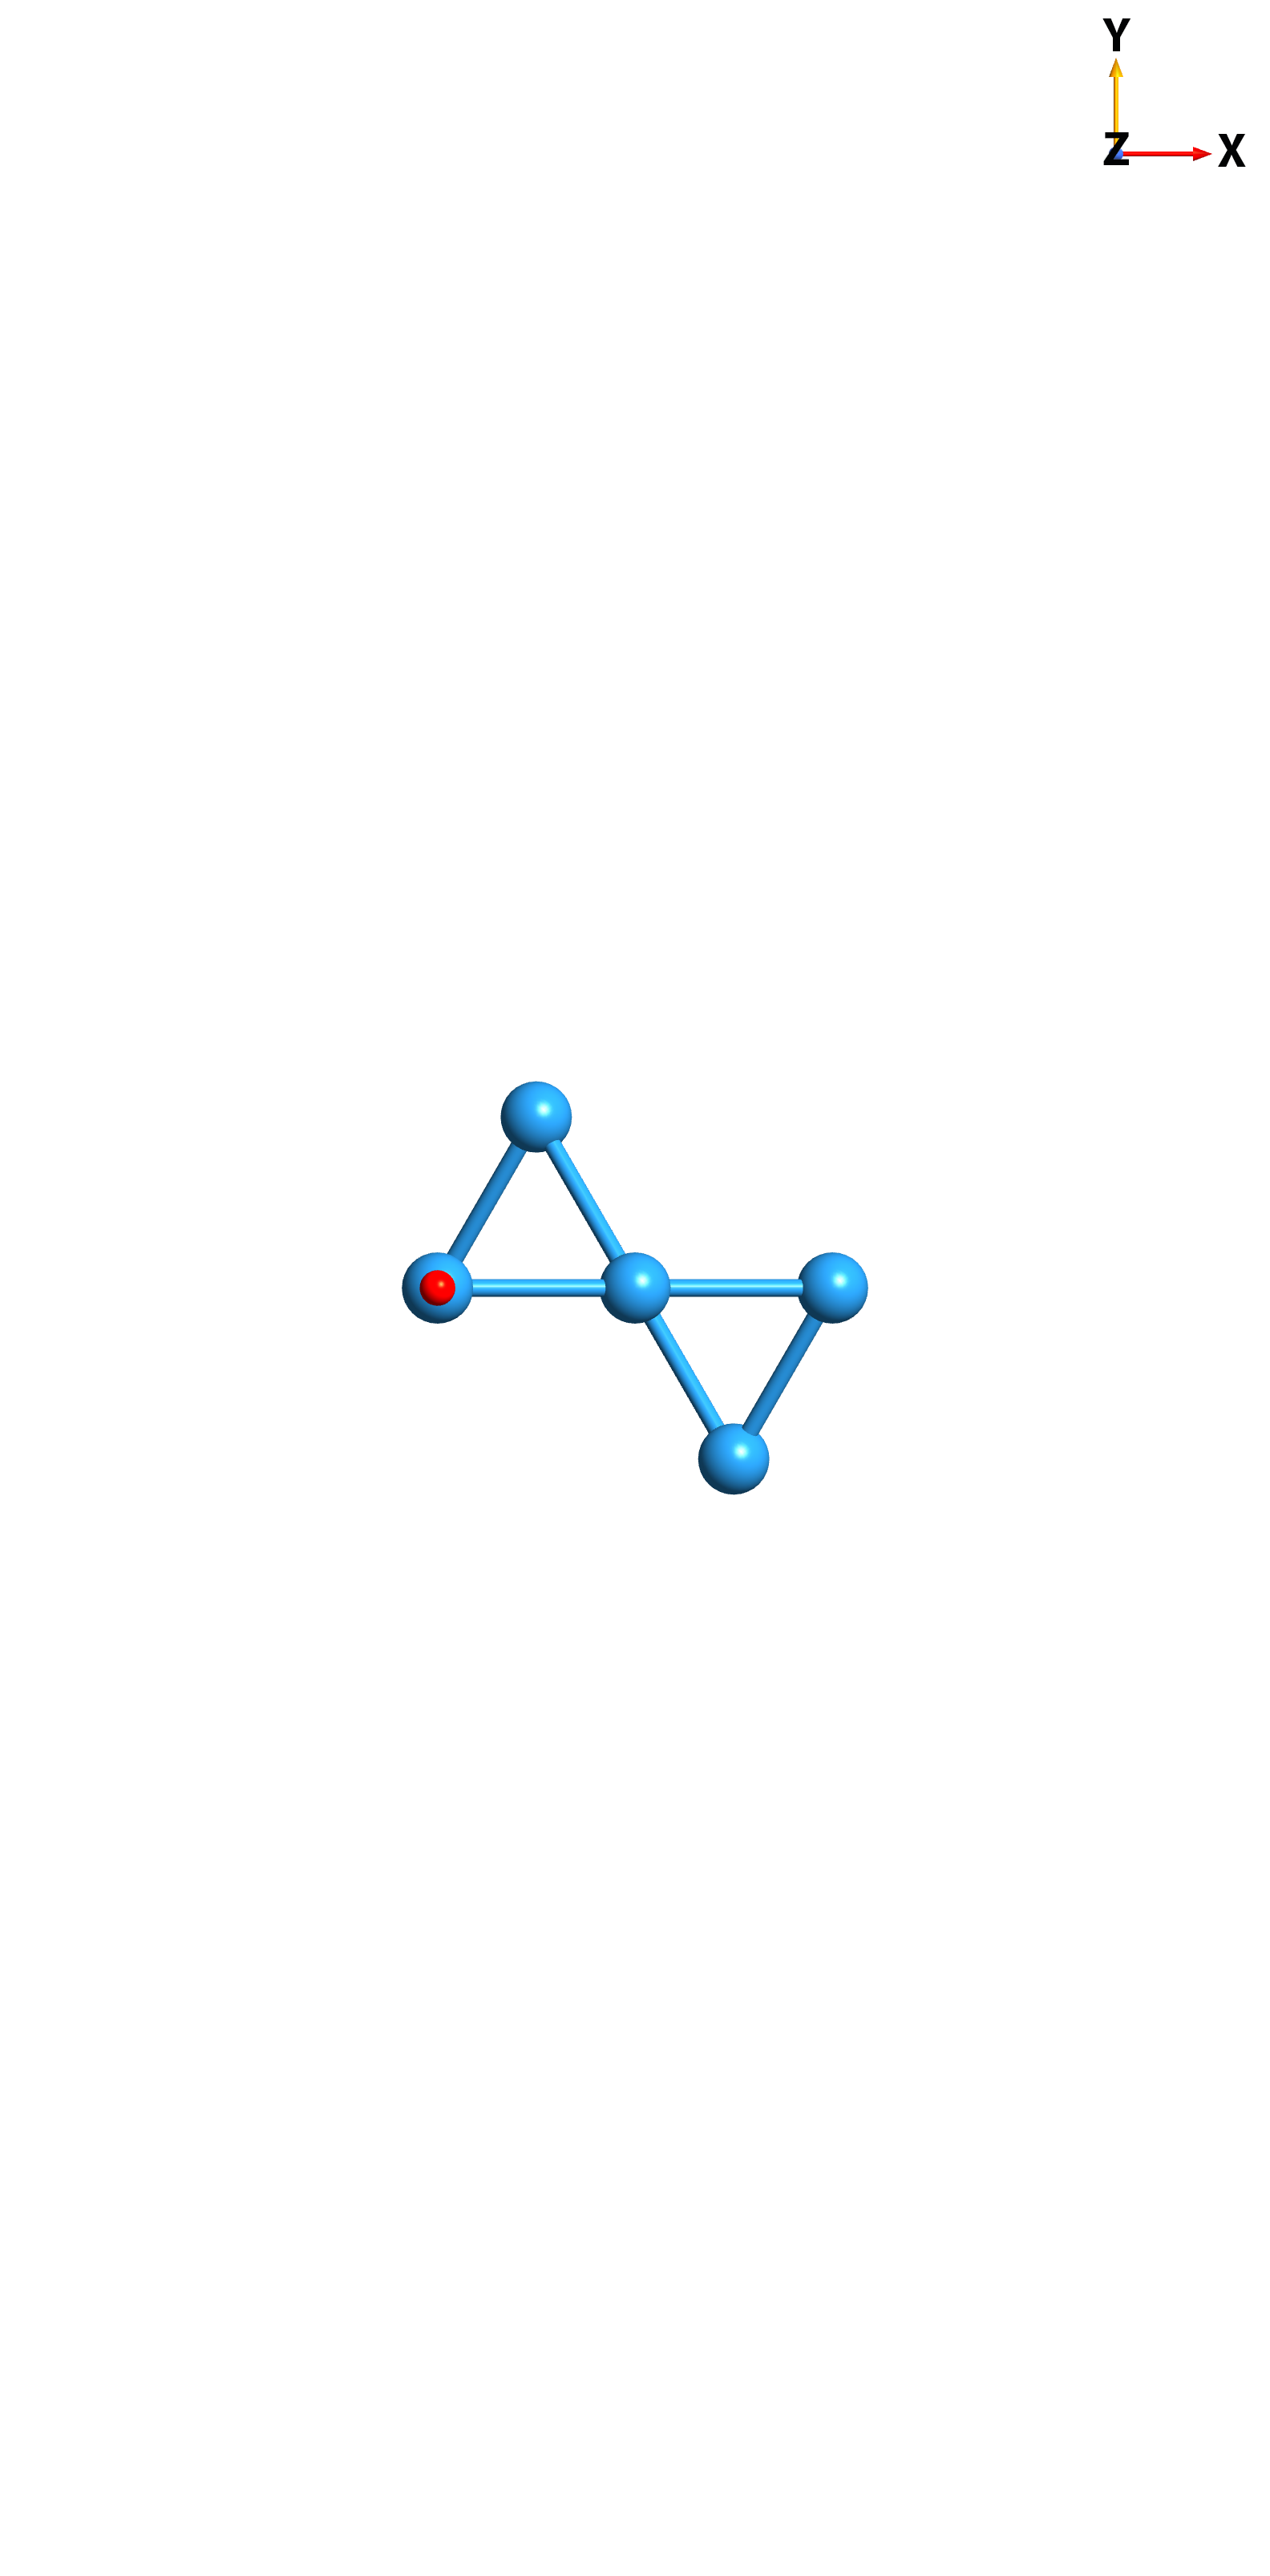
\includegraphics[width=0.3\textwidth]{content/figures/struc-Si1x1-top}}
\caption[Several views of the slab used to represent the Si(111)(1$\times$1):H
surface.]
{Several views of the slab used to represent the Si(111)(1$\times$1):H
surface. This particular slab has 16 Si atomic layers (large blue balls) with
two H atomic layers (small red balls).}
\label{fig:1x1struc}
\end{figure}

The electronic wave-functions, $\psi_{n\mathbf{k}}(\mathbf{r})$, were also
calculated with the ABINIT code using a planewave basis set with an energy
cutoff of 15 Hartrees. $\chi^{\mathrm{abc}_{\mathrm{surface}}}$ was properly
converged with 576 \textbf{k} points in the irreducible Brillouin zone, which
are equivalent to 1250 \textbf{k} points when disregarding symmetry relations.
The contribution of $\mathbf{v}^\mathrm{nl}$ in Eq. \eqref{eq:chis} was carried
out using the DP \cite{olevanoDP} code implemented in TINIBA \cite{tiniba}, with
a basis set of 3000 planewaves. Convergence for the number of bands was achieved
at 200, which includes 97 occupied bands and 103 unoccupied bands. All spectra
were produced using a scissors value of 0.7 eV in the
$\chi^{\mathrm{abc}_{\mathrm{surface}}}$ and
$\boldsymbol{\epsilon}_{\ell}(\omega)$ calculations. This value was obtained
from Ref. \cite{liPRB10}, in which the authors carry out a
$\mathrm{G}_{0}\mathrm{W}_{0}$ calculation on this surface for increasing
numbers of layers. They calculated the LDA and $\mathrm{G}_{0}\mathrm{W}_{0}$
band gaps, and found that the difference between the two tends towards $\sim0.7$
eV as more layers are added, culminating in a value of 0.68 eV for bulk Si. This
calculation is completely \emph{ab-initio}, so I consider 0.7 eV to be a very
reasonable value for the scissors correction.

It is important to mention that we must also calculate the bulk and surface
dielectric functions, $\boldsymbol{\epsilon}_b(\omega)$ and
$\boldsymbol{\epsilon}_\ell(\omega)$. For this, we follow the method presented
in Ref. \cite{mendozaPRB06}. For the bulk, the tensor components are equal in
all three directions due to the cubic symmetry,
\begin{equation*}
\varepsilon_{b}(\omega) = 
\epsilon^{xx}_{b}(\omega) = 
\epsilon^{yy}_{b}(\omega) = 
\epsilon^{zz}_{b}(\omega).
\end{equation*}
For the purpose of this calculation, we introduce the average value for the
surface dielectric function, $\varepsilon_\ell(\omega)$. This entails that
$\epsilon^{xx}_{\ell}(\omega) = \epsilon^{yy}_{\ell}(\omega) \approx
\epsilon^{zz}_{\ell}(\omega)$, since symmetry is broken in the $zz$ direction
because of the surface. We find the average in the conventional way,
\begin{equation*}
\varepsilon_{\ell}(\omega) = 
\frac{\epsilon^{xx}_{\ell}(\omega) + 
\epsilon^{yy}_{\ell}(\omega) + 
\epsilon^{zz}_{\ell}(\omega)}{3},
\end{equation*}
and use that quantity in the equations for the SSHG yield. In order to obtain a
result which does not depend on the size of the vacuum region
\cite{nicolasPRB15}, we have normalized the surface dielectric function to the
volume of the slab, instead of the volume of the super-cell. We remark that we
could calculate $\epsilon^{\mathrm{ab}}_{\mathrm{half-slab}}(\omega)$ using
${\mathcal{C}}(z)=1$ for the upper half of our slab and normalize to the volume
of the half-slab. Nevertheless, $\epsilon^{\mathrm{ab}}_{\ell}(\omega)$ and
$\epsilon^{\mathrm{ab}}_{\mathrm{half-slab}}(\omega)$ give the same
result \cite{hoganPRB03, castilloPRB03, nicolasPRB15}.

%%%%%%%%%%%%%%%%%%%%%%%%%%%%%%%%%%%%%%%%%%%%%%%%%%%%%%%%%%%%%%%%%%%%%%%%%%%%%%%%

\subsection{Calculating 
\texorpdfstring{$\chi^{xxx}_{\mathrm{surface}}(-2\omega;\omega,\omega)$}{Xxxx}}
\label{sec:res1x1chi}

The pioneering work presented in Ref. \cite{mejiaPRB02} showed the effect of
artificially moving the atomic position on the resulting SSHG spectra. In this
section, I will address the more practical and relevant case of atomic
relaxation. More precisely, I compare the fully relaxed structure described
above with an unrelaxed structure where all the Si atoms are at the ideal bulk
positions. Note that in both cases, the Si-H bond distance is the same 1.5\,\AA.
The unrelaxed coordinates use the same parameters mentioned above. Fortunately,
there exists experimental data that can be compared to the calculated
$\chi^{xxx}_{\mathrm{surface}}$ for this surface, taken from Ref.
\cite{hoferAPA96}. This data provides an excellent point of comparison as it was
presented in absolute units and was measured at a very low temperature of 80 K.

Fig. \ref{fig:Xxxx} depicts the spectra from the relaxed and unrelaxed
coordinates compared to experiment. The theoretical curves were calculated with
a scissors shift of $\hbar\Delta = 0.7$ eV, as mentioned in the previous
section. The relaxed coordinates have a peak position that is very slightly
blueshifted with respect to the experimental peak near 1.7 eV. In contrast, the
unrelaxed coordinates have a peak that is redshifted close to 0.05 eV from
experiment. There is also a feature between 1.5 eV and 1.6 eV that appears in
the relaxed spectrum that coincides partially with the experimental data. Both
theoretical curves have half the intensity of the experimental peak. It is
important to note that this data was taken at low temperature (80 K); this
further favors the comparison, as the theory neglects the effects of
temperature. As is shown in Ref. \cite{hoferAPA96}, the peaks in the spectrum
redshift as the temperature increases. Intensity for both the relaxed and
unrelaxed curves are roughly half the intensity of the experimental spectrum. I
have converted the units of the experimental data from CGS to MKS units for
easier comparison.

\begin{figure}[t]
\centering
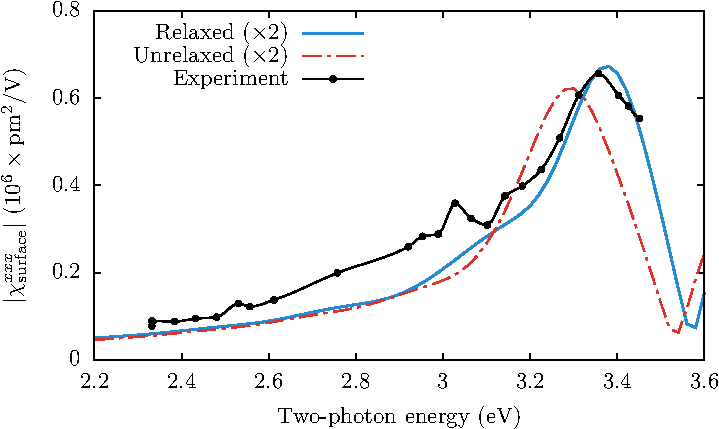
\includegraphics[width=0.6\textwidth]{content/figures/fig-Si1x1-Hofer_Xxxx}
\caption[$\chi^{xxx}_{\mathrm{surface}}$ calculated using relaxed and unrelaxed
atomic positions.]
{Comparison of $\chi^{xxx}_{\mathrm{surface}}$ calculated using relaxed and
unrelaxed atomic positions, with the experimental data presented in Ref.
\cite{hoferAPA96}. The theoretical curves were calculated with a scissors shift
of $\hbar\Delta = 0.7$ eV, and are broadened with $\sigma=0.075\,\text{eV}$.
Experimental data was taken at 80 K.}
\label{fig:Xxxx}
\end{figure}

We can conclude that the most accurate theoretical results are produced by using
relaxed atomic positions for the calculation of
$\boldsymbol{\chi}_{\mathrm{surface}}$. Although this process can be very time
consuming for large numbers of atoms, this should be considered a crucial step.
This also further demonstrates that SSHG is very sensitive to the surface atomic
positions. In particular, these results show that a correct value of the Si-H
bond length is not enough to obtain the most accurate SSHG spectra, and that a
full relaxation of the structure is required. Additionally, it seems that the
theory may coincide better with experiments that are conducted under very low
temperature conditions.


%%%%%%%%%%%%%%%%%%%%%%%%%%%%%%%%%%%%%%%%%%%%%%%%%%%%%%%%%%%%%%%%%%%%%%%%%%%%%%%%
%%%%%%%%%%%%%%%%%%%%%%%%%%%%%%%%%%%%%%%%%%%%%%%%%%%%%%%%%%%%%%%%%%%%%%%%%%%%%%%%

\subsection{Comparing the Theoretical \texorpdfstring{$\mathcal{R}$}{R} to
Experiment}
\label{sec:1x1sshgyield}

All calculations presented from this point on were done using the relaxed atomic
positions described in the the previous section. I will now present the
theoretical SSHG yield for the Si(111)(1$\times$1):H surface compared to
experiments from Refs. \cite{mitchellSS01, mejiaPRB02, bergfeldPRL04}. These
comparisons are good benchmarks to test the complete formalism for calculating
the SSHG yield.

The method of calculation is as follows. I first calculated
$\varepsilon_{b}(\omega)$, $\varepsilon_{\ell}(\omega)$, and then
$\chi^{\mathrm{abc}}_{\mathrm{surface}}$ from Eq. \eqref{eq:chis}. I used these
for the Fresnel factors and in Eqs. \eqref{eq:rpp111}, \eqref{eq:rps111}, and
\eqref{eq:rsp111}, and finally, those into Eq. \eqref{eq:mc6} to obtain the
theoretical SSHG yield for different polarizations that can then be compared
with the experimental data. Remember that a scissors shift of $\hbar\Delta =
0.7$ eV is used for all the $\chi^{\mathrm{abc}}_{\mathrm{surface}}$ components.
These components and the calculated ${\mathcal{R}}$ spectra were also broadened
with a Gaussian broadening of $\sigma=0.075$ eV. These values were selected so
that the theoretical calculation best represents the lineshape of the
experimental spectrum.


%%%%%%%%%%%%%%%%%%%%%%%%%%%%%%%%%%%%%%%%%%%%%%%%%%%%%%%%%%%%%%%%%%%%%%%%%%%%%%%%

\subsubsection{Overview of the calculated \texorpdfstring{$\mathcal{R}$}{R}
spectra}\label{sec:1x1R3D}

We will carefully explain and compare the calculated $\mathcal{R}$ for each
different polarization case in the following sections. However, I first want to
present a general overview of the theoretical SSHG yield, as I did in Sec.
\ref{sec:2x1R3D}. In Figs. \ref{fig:1x1rP3d} and \ref{fig:1x1rS3d}, I present
these results over a two-photon energy range of 2.5-5 eV. This range corresponds
to the experimental measurements featured in Refs. \cite{mejiaPRB02} and
\cite{bergfeldPRL04}. Note that the SSHG yield drops to zero very rapidly before
for energy values under 3 eV. This is because of the lack of surfaces states due
to the surface H-saturation.

\begin{figure}[t]
\centering
\subbottom[$\mathcal{R}_{pP}$\label{fig:1x1rpp3d}]%
{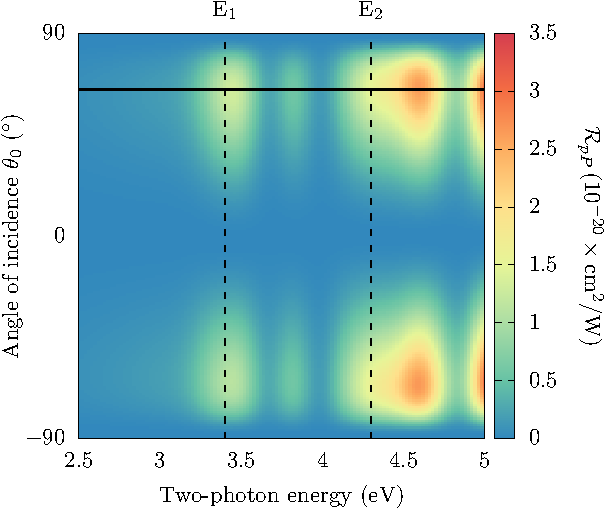
\includegraphics[height=0.39\textwidth]{content/figures/3D-Si1x1-RpP}}\hfill
\subbottom[$\mathcal{R}_{sP}$\label{fig:1x1rsp3d}]%
{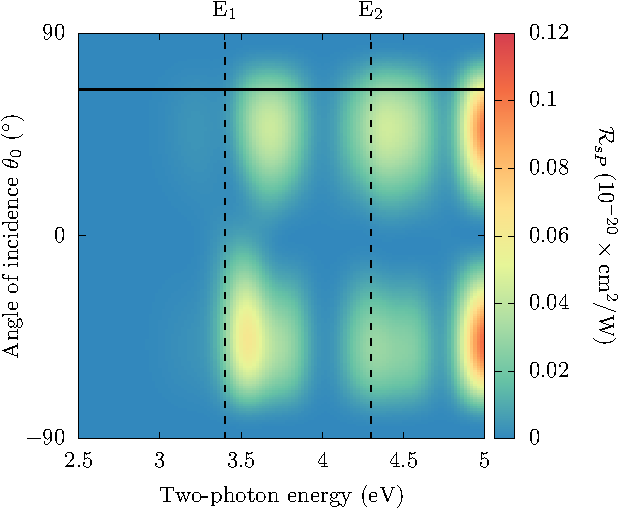
\includegraphics[height=0.39\textwidth]{content/figures/3D-Si1x1-RsP}}
\caption[Overview of the angular dependence of $\mathcal{R}_{\mathrm{iP}}$.]
{$\mathcal{R}$ for outgoing $P$ polarization, versus the angle of
incidence ($\theta_{0}$) for the Si(111)(1$\times$1):H surface. A scissors shift
of $\hbar\Delta = 0.7$ eV is applied. The solid line represents $\theta_{0} =
65^{\circ}$, and the dotted lines represent the E$_{1}$ and E$_{2}$ Si critical
points. Both figures consider an azimuthal angle of $\phi = 30^{\circ}$.}
\label{fig:1x1rP3d}
\end{figure}

I have included some helpful markers in these figures. First, the solid black
line represents an angle incidence of $\theta_{0} = 65^{\circ}$. This is one of
two angles that we will consider for the remainder of this chapter; in
particular, this is the angle used in the experiment from Ref. Refs.
\cite{mejiaPRB02}. It is clear that they chose this particular angle to maximize
the $\mathcal{R}_{pP}$ output. Second, the dashed black lines represent the
$E_{1} = 3.4$ eV and $E_{2} = 4.3$ eV critical points of bulk Si
\cite{yubook}. For the outgoing $P$ polarization in Fig. \ref{fig:1x1rP3d}, we
can see that the calculated SSHG yield does have peaks around those energy
values. We will review this in much further detail below. We see similar
characteristics, for Fig. \ref{fig:1x1rS3d} with the outgoing $S$ polarization
cases. Indeed, the theoretical peak values seem to match quite well with the
critical points. Again, we will review these findings in much more detail below.
Note that I will omit $\mathcal{R}_{sS}$ from this point forward, as I do not
have any experimental data to compare it with.

\begin{figure}[H]
\centering
\subbottom[$\mathcal{R}_{pS}$\label{fig:1x1rps3d}]%
{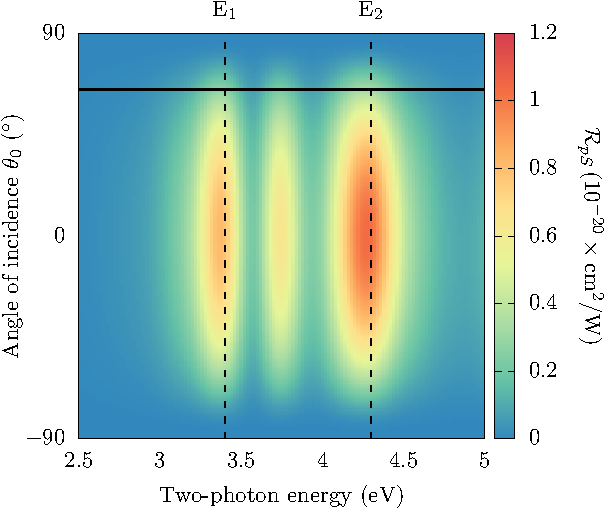
\includegraphics[height=0.39\textwidth]{content/figures/3D-Si1x1-RpS}}\hfill
\subbottom[$\mathcal{R}_{sS}$\label{fig:1x1rss3d}]%
{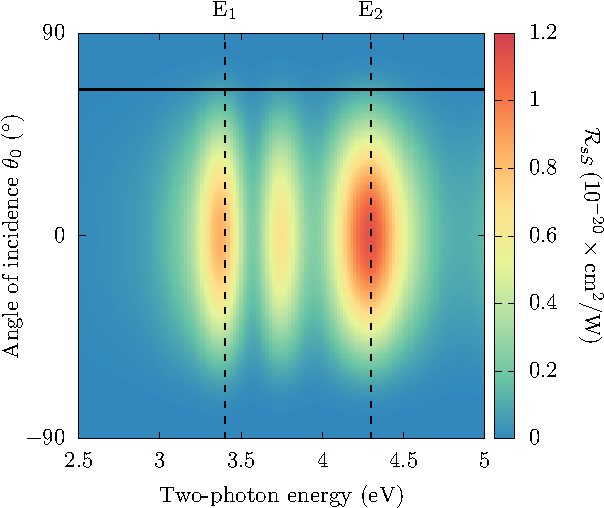
\includegraphics[height=0.39\textwidth]{content/figures/3D-Si1x1-RsS}}
\caption[Overview of the angular dependence of $\mathcal{R}_{\mathrm{iS}}$.]
{$\mathcal{R}$ for outgoing $S$ polarized fields, versus the angle of
incidence ($\theta_{0}$) for the Si(111)(1$\times$1):H surface. A scissors shift
of $\hbar\Delta = 0.7$ eV is applied. The solid line represents $\theta_{0} =
65^{\circ}$, and the dotted lines represent the E$_{1}$ and E$_{2}$ Si critical
points. Both figures consider an azimuthal angle of $\phi = 30^{\circ}$.}
\label{fig:1x1rS3d}
\end{figure}


%%%%%%%%%%%%%%%%%%%%%%%%%%%%%%%%%%%%%%%%%%%%%%%%%%%%%%%%%%%%%%%%%%%%%%%%%%%%%%%%

\subsubsection{\texorpdfstring{$\mathcal{R}_{pP}$}{RpP}($p$-in, $P$-out)}
\label{sec:1x1RpP}

We first analyze how the inclusion of multiple reflections affects the
calculated SSHG yield. I will conduct this study for $\mathcal{R}_{pP}$ as it is
typically associated with the strongest signal output. It is also by far the
most involved calculation out of the four different polarization cases, since it
includes all four nonzero components. We are interested in finding the thickness
of the layer $\ell$ where $\chi^{\mathrm{abc}}_{\mathrm{surface}} \ne 0$. As
mentioned above, we found reasonable converged results for this surface using a
slab of 48 atomic layers. This corresponds to a thickness of $\sim 5$ nm, that
is equivalent to the 24 atomic sheets of Si along the (111) direction,
corresponding to the half-slab. As this represents only the upper half of the
slab, we find it reasonable to choose the thickness of the layer $\ell$ to be
between $d\sim 5-10$ nm, as in this range of values
$\chi^{\mathrm{abc}}_{\mathrm{surface}}$ will be well converged.

We begin our comparisons in Fig. \ref{fig:average}, in which we compare the
theoretical results for the SHG radiation with the experimental results from
Ref. \cite{mejiaPRB02}. First, we note that the experimental spectrum shows two
very well defined resonances which come from electronic transitions from the
valence to the conduction bands around the well known $E_{1}\sim 3.4$ eV and
$E_{2}\sim 4.3$ eV critical points of Si \cite{yubook}. We mention that the
experimental results where produced with an angle of incidence of
$\theta=65^\circ$, and an azimuthal angle of $\phi=30^\circ$, which eliminates
the contribution from $\chi^{xxx}_{\mathrm{surface}}$ from Eq.
\eqref{eq:rpp111}. The theoretical curves that include multiple reflections are
featured with the average value $\bar{R}^{M}_{p}$, Eq.
\eqref{eq:mcave}, with two values for the total thickness, $d$, and Eqs.
\eqref{eq:mc78} and \eqref{eq:rpp111}. We contrast these with the standard three
layer model excluding the effects of multiple reflections from Sec.
\ref{sec:nomr}. We see that the $E_{2}$ peak is blueshifted by around 0.3 eV,
and the yield does not go to zero after 4.75 eV. We can attribute these
shortcomings to the fact that both $\chi^{zzz}_{\mathrm{surface}}$ and
$\chi^{xxz}_{\mathrm{surface}}$ include out-of-plane incoming fields. These are
affected by local field effects that can change both intensity and peak position
\cite{tancognedejean:tel-01235611}. Including these effects is computationally
very expensive and is beyond the scope of this work. We speculate that the
components of $\chi^{abc}_{\mathrm{surface}}$ necessary for $\mathcal{R}_{pP}$
require the proper inclusion of these effects in order to accurately describe
the experimental peaks. Additionally, Ref. \cite{dadapPRB97} shows that low
temperature measurements of $\mathcal{R}_{pP}$ will blueshift the spectrum away
from room temperature measurements such as those shown in Figs. \ref{fig:RpP}
and \ref{fig:mitchellRpP}, and towards the theoretical results.

\begin{figure}[t]
\centering
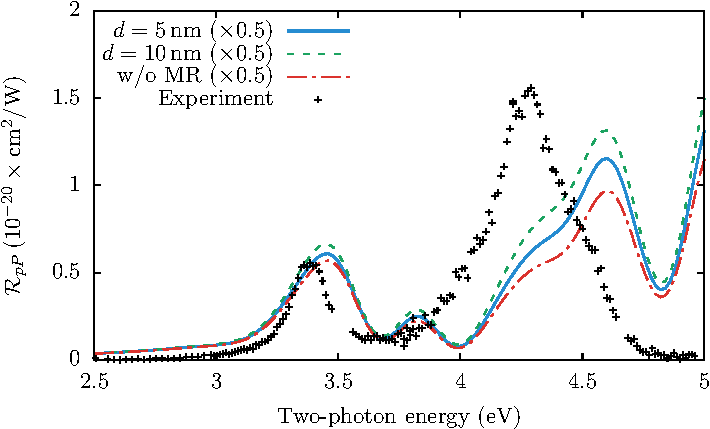
\includegraphics[width=0.7\textwidth]{content/figures/fig-Si1x1-MRthickness}
\caption{$\mathcal{R}_{pP}$ for two thickness values $d$ of the thin layer
$\ell$.}
{Comparison between the three layer model with the effects of multiple
reflections for two different values of the total layer thickness $d$, with the
standard three layer model without the effects of multiple reflections, and the
experimental data from Ref. \cite{mejiaPRB02}. We take $\theta=65^{\circ}$,
$\phi=30^{\circ}$, and a scissors value of $\hbar\Delta = 0.7\,\text{eV}$.}
\label{fig:average}
\end{figure}

We can see that including the effects of multiple reflections enhances the
E$_{2}$ peak significantly, and that the enhancement increases with the
thickness $d$ of the thin layer $\ell$. This should be quite obvious from
\ref{fig:MR3layer2w}; as the layer thickness increases, so does the total
contribution from the multiple reflections. Since we have already established
that using a layer thickness of 10 nm is reasonable for this surface, I will use
this value from this point on.

In Fig. \ref{fig:mr21w}, I present the results from calculating the spectra with
and without the multiple reflections from the $1\omega$ fields. The difference
between the two lines is almost negligible for energies below 4 eV. After 4 eV,
the spectrum without the $1\omega$ multiple reflections is less intense. The
difference in intensity between the two curves is most noticeable at E$_{2}$. We
can conclude that the $1\omega$ multiple reflections contribute only slightly to
the region around E$_{2}$, and are almost negligible elsewhere. This is clear
since the phase shift of Eq. \eqref{mphi} is not only a factor of 2 smaller than
that of Eqs. \eqref{eq:delta0} and \eqref{eq:delta}, but also $w_\ell < W_\ell$.
However, including them is indeed necessary in order to have the most complete
formulation, and calculating $r^{M}_{p}$ comes at no additional computational
expense.

\begin{figure}[t]
\centering
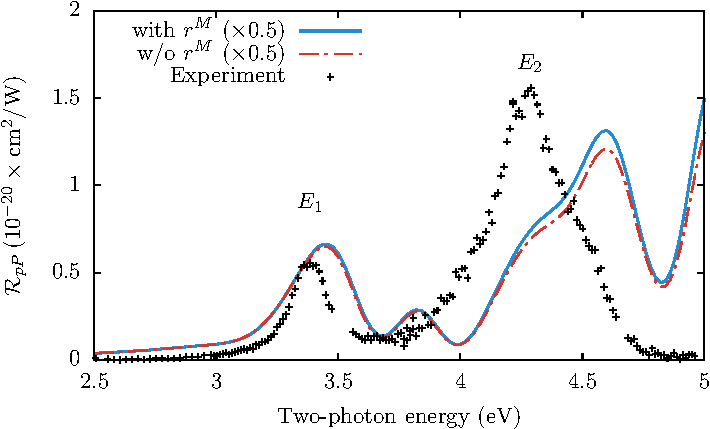
\includegraphics[width=0.7\textwidth]{content/figures/fig-Si1x1-MRno1w}
\caption[Including or neglecting the effects of multiple reflections for the
fundamental fields]
{Comparison between including or neglecting the effects of multiple
reflections for the fundamental fields. The theoretical spectra were produced
for a layer thickness of $d = 10$ nm using the average value of
$\bar{R}^{M}_{p}$.}
\label{fig:mr21w}
\end{figure}

We can analyze the effects of moving the polarization sheet to different depths
within the layer $\ell$ in Fig. \ref{fig:d2values}. As mentioned above, we
consider a layer thickness of $d = 10$ nm. We compare the theoretical SSHG yield
for $d_{2} = 0$ nm and $d_{2} = 10$ nm, with the SSHG yield that neglects
multiple reflections. When $d_{2} = 0$ nm, we have placed the polarization sheet
at the bottom of the layer region. This minimizes the effect of the multiple
reflections, and thus the curve is very similar to the three layer model that
neglects multiple reflections entirely. When $d_{2} = 10$ nm, the polarization
sheet is placed at the top of the layer region. This maximizes the effect of the
multiple reflections and therefore leads to the largest yield. We also notice
that the average value obtained by using $\bar{R}^{M}_{p}$ (Eq.
\eqref{eq:mcave}) is intermediate between $d_{2} = 0$ and $d_{2} = 10$ nm, as
expected. This is very similar to selecting $d_{2} = d/2$, which can be
interpreted as placing the nonlinear polarization sheet
$\mathbf{P}(\mathbf{r},t)$ at the middle of the thin layer $\ell$.

As before, these enhancements are larger for $E_{2}$ than for $E_{1}$. This can
be understood from the fact that the corresponding $\lambda_{0}$ for $E_{1}$ is
larger than that of $E_{2}$. From Eqs. \eqref{eq:delta0}, \eqref{eq:delta}, and
\eqref{mphi}, we see that the phase shifts are larger for $E_{2}$ than for
$E_{1}$, producing a larger enhancement of the SSHG yield at $E_{2}$ from the
multiple reflections. As the phase shifts grow with $d$, so does the enhancement
caused by the multiple reflections. From this figure, it becomes evident that
the inclusion of multiple reflections is crucial to obtain a better agreement
between the theoretical SSHG yield and the experimental spectrum. This is
particularly true for larger energies, such as $E_{2}$, as $\lambda_{0}$ becomes
smaller and the multiple reflection effects become more noticeable. The selected
value for $d << \lambda_{0}$, that comes naturally from the \emph{ab initio}
calculation of $\chi^{\mathrm{abc}}_{\mathrm{surface}}$ is thus very reasonable
in order to model a thin surface layer below the vacuum region where the
nonlinear SH conversion takes place. From this point on, we will always include
the effects of multiple reflections in the 3-layer model, with a layer thickness
of $d = 10$ nm and the average value of $\bar{R}^{M}_{p}$.

\begin{figure}[H]
\centering
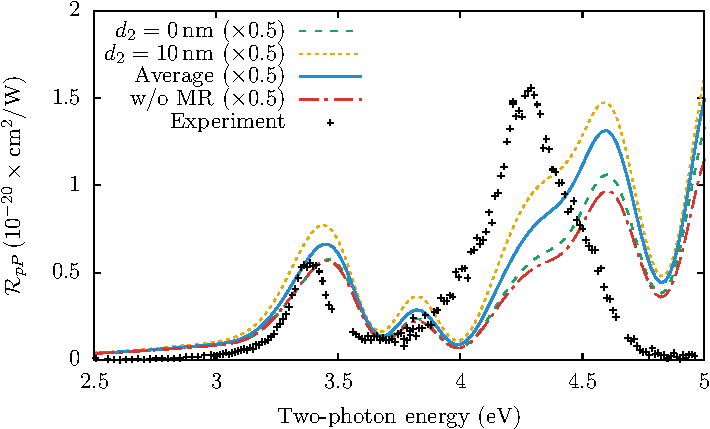
\includegraphics[width=0.7\textwidth]{content/figures/fig-Si1x1-MRdepth}
\caption[Different depths for the placement of the polarization sheet in the
thin layer $\ell$.]
{Comparison between the three layer model with the effects of multiple
reflections for two different values of $d_{2}$, and the average value
$\bar{R}^{M}_{p}$. All curves that include multiple reflections consider a layer
$\ell$ thickness of $d = 10\,\mathrm{nm}$.}
\label{fig:d2values}
\end{figure}

I will now present an overview of the different models from Sec.
\ref{sec:scenarios}, and summarized in Table \ref{tab:models}. Namely, we will
compare the 3-layer model with multiple reflections, the 2-layer-fresnel,
2-layer-bulk, 2-layer-vacuum, and 3-layer hybrid models. In Fig. \ref{fig:RpP},
I present a comparison between the 3-layer, 3-layer-hybrid, and 2-layer-bulk
models with experiment. The peak position for the 3-layer model compares quite
nicely to the experimental peaks, with an overall intensity that is only two
times larger. The 2-layer-bulk model is almost identical in lineshape to the
3-layer model, but with four times less intensity than the experiment. The
3-layer-hybrid model is also similar in lineshape with a less pronounced E$_{2}$
peak, and is half as intense as the experiment. All these observations are
consistent as $\epsilon_{b}$ and $\epsilon_{\ell}$ differ mostly in intensity;
each model is screened with either $\epsilon_{b}$ (2-layer-bulk),
$\epsilon_{\ell}$ (3-layer), or a combination of the two (3-layer-hybrid).
Ultimately, the 3-layer model has better peak proportions and good intensity,
but the other two models are interesting alternatives.

\begin{figure}[t]
\centering 
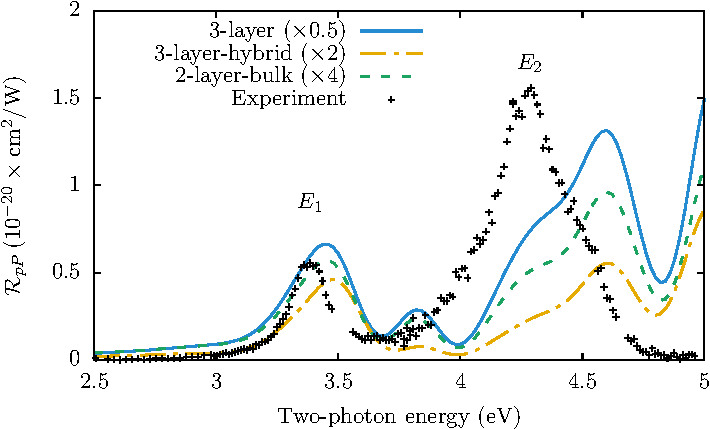
\includegraphics[width=0.7\textwidth]{content/figures/fig-Si1x1-Mejia_RpP}
\caption[$\mathcal{R}_{pP}$ compared to experimental data from Mejia et al.]
{Comparison between theoretical models (see Table \ref{tab:models}) and
experiment for $\mathcal{R}_{pP}$, for $\theta=65^{\circ}$, and a scissors value
of $\hbar\Delta = 0.7\,\text{eV}$. Experimental data taken from Ref. 
\cite{mejiaPRB02}, measured at room temperature.}
\label{fig:RpP}
\end{figure}

The two remaining models from Sec. \ref{sec:scenarios} are presented in Fig.
\ref{fig:othermodels}. The 2-layer-fresnel model produces a spectrum with peak
positions that are close to the experiment, but are around 40 times more
intense. The calculated E$_{2}$ peak is similar, but the E$_{1}$ peak lacks the
sharpness present in the experiment, with poor proportional intensity between
the peaks. On the other hand, the 2-layer-vacuum model has the most extreme
intensity difference with the experiment, over 5 orders of magnitude higher. The
lineshape reproduces the E$_{2}$ peak quite well, but lacks a sharp E$_{1}$ peak
with poor peak position. Clearly, the screening provided by $\epsilon_{b}$ and
$\epsilon_{\ell}$ are necessary for accurate results. From Eq.
\eqref{eq:rpp111}, it is clear that $\mathcal{R}_{pP}$ has several $2\omega$
terms that will change between models; this will have a deep effect on the
lineshape. Additionally, $\Gamma^{\ell}_{pP}$ also has
$\varepsilon_{\ell}(2\omega)$ in the denominator, and so we have a significant
difference in both lineshape and intensity between these models and the rest.

From this point forward, we will only consider the 3-layer (with multiple
reflections), the 2-layer-fresnel (the historically popular model), and the
2-layer bulk models. These three models give an interesting overview of the
different possibilities available and add some insight into the physics behind
the SSHG yield.

\begin{figure}[H]
\centering 
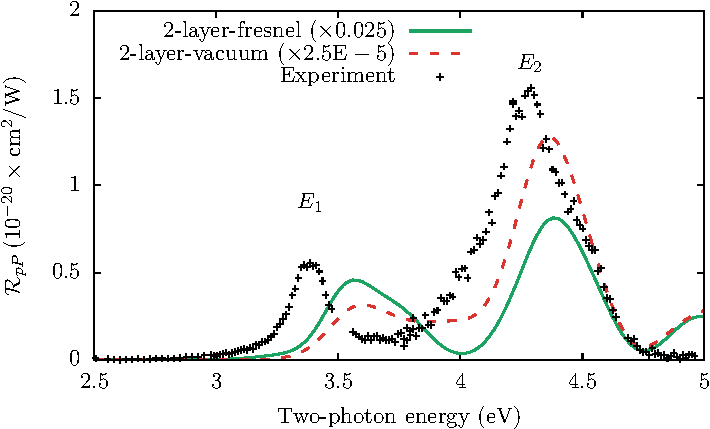
\includegraphics[width=0.7\textwidth]
{content/figures/fig-Si1x1-Mejia_RpP_models}
\caption[2-layer-fresnel and 2-layer vacuum for $\mathcal{R}_{pP}$.]
{Comparison between the 2-layer-fresnel and 2-layer-vacuum models (see Table
\ref{tab:models}) and experiment for $\mathcal{R}_{pP}$, for
$\theta=65^{\circ}$, and a scissors value of $\hbar\Delta = 0.7\,\text{eV}$.
Experimental data taken from Ref. \cite{mejiaPRB02}, measured at room
temperature.}
\label{fig:othermodels}
\end{figure}

In Fig. \ref{fig:mitchellRpP}, I compare the theoretical spectra to results from
Ref. \cite{mitchellSS01}. The 3-layer model is, as before, close to the
experiment in both peak position and intensity. Intensity is almost the same the
experimental value. This provides a more compelling argument against the
2-layer-fresnel model than Fig. \ref{fig:RpP}. The 2-layer-fresnel model is 20
times more intense and blueshifted by around 0.1 eV. As mentioned above, this
surface is of very high quality with measurements taken shortly after surface
preparation. The 2-layer-bulk model is intermediate between the other two models
in both intensity and lineshape. Under these conditions, the 3-layer model very
accurately reproduces the E$_{1}$ peak over the 2-layer-fresnel and 2-layer-bulk
models.

\begin{figure}[t]
\centering
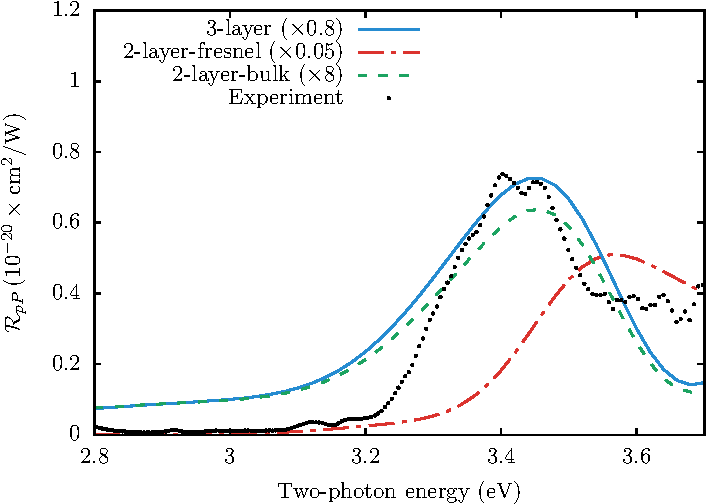
\includegraphics[width=0.7\textwidth]{content/figures/fig-Si1x1-Mitchell_RpP}
\caption[$\mathcal{R}_{pP}$ compared to experimental data from Mitchell et al.]
{Comparison between theoretical models (see Table \ref{tab:models}) and
experiment for $\mathcal{R}_{pP}$, for $\theta=45^{\circ}$, and a scissors value
of $\hbar\Delta = 0.7\,\text{eV}$. Experimental data taken from Ref.
\cite{mitchellSS01}, measured at room temperature.}
\label{fig:mitchellRpP}
\end{figure}


%%%%%%%%%%%%%%%%%%%%%%%%%%%%%%%%%%%%%%%%%%%%%%%%%%%%%%%%%%%%%%%%%%%%%%%%%%%%%%%%

\subsubsection{Calculated \texorpdfstring{$\mathcal{R}_{sP}$}{RsP} compared to 
experiment}\label{sec:1x1RsP}

Next, we will compare the calculated $\mathcal{R}_{sP}$ spectra with
experimental data from Ref. \cite{mejiaPRB02}. The calculation adheres to the
experimental setup by taking an angle of incidence $\theta=65^{\circ}$ and an
azimuthal angle $\phi=30^\circ$. As seen in Fig. \ref{fig:RsP}, the overall
intensity of $\mathcal{R}_{sP}$ is one order of magnitude lower than
$\mathcal{R}_{pS}$. The experimental data is far noisier than in the other cases
but the E$_{1}$ and E$_{2}$ peaks are still discernible. As with the previous
comparisons, the 3-layer model is the closest match in both intensity and
lineshape to the experimental spectrum. It produces a curve that is very close
to the experimental intensity with good proportional heights for the calculated
E$_{1}$ and E$_{2}$ peaks. In contrast, the 2-layer-fresnel model is 100 times
more intense than experiment and produces an enlarged E$_{2}$ peak. The
2-layer-bulk model is ten times smaller with a very similar lineshape to the
3-layer model.

The differences between the 2-layer-fresnel and 2-layer-bulk models are not
derived from Eq. \eqref{eq:rsp111}, as the $\varepsilon_{b}(2\omega)$ does not
change and the second term vanishes for this azimuthal angle of $\phi = 30$.
However, $\Gamma^{\ell}_{sP}$ does cause a significant change in the intensity
as there is an $\varepsilon_{\ell}(2\omega)$ term in the denominator. This will
become $\varepsilon_{v}(2\omega) = 1$ for the 2-layer-fresnel model, and
$\varepsilon_{b}(2\omega)$ in the bulk model. This accounts for the significant
difference between the intensity of the two models, while the lineshape remains
mostly consistent. At higher energies, the theoretical curve is blueshifted as
compared to the experiment. The best explanation for this is the inclusion of
the scissor operator, which does not adequately correct the transitions
occurring at these higher energies. A full GW calculation would be well suited
for this task, but is well beyond the scope of this work.

\begin{figure}[t]
\centering
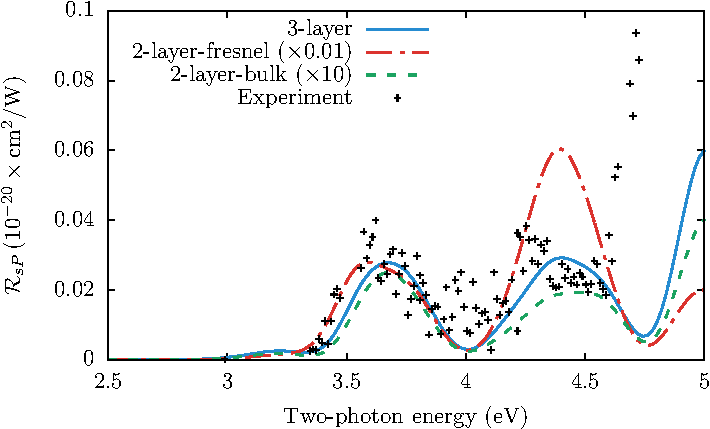
\includegraphics[width=0.7\textwidth]{content/figures/fig-Si1x1-Mejia_RsP}
\caption[$\mathcal{R}_{sP}$ compared to experimental data from Mejia et al.]
{Comparison between theoretical models (see Table \ref{tab:models}) and
experiment for $\mathcal{R}_{sP}$, for $\theta=65^{\circ}$, and a scissors value
of $\hbar\Delta = 0.7\,\text{eV}$. Experimental data taken from Ref.
\cite{mejiaPRB02}, measured at room temperature.}
\label{fig:RsP}
\end{figure}


%%%%%%%%%%%%%%%%%%%%%%%%%%%%%%%%%%%%%%%%%%%%%%%%%%%%%%%%%%%%%%%%%%%%%%%%%%%%%%%%

\subsubsection{Calculated \texorpdfstring{$\mathcal{R}_{pS}$}{RpS} compared to 
experiment}\label{sec:1x1RpS}

We will now compare the $\mathcal{R}_{pS}$ spectra with room temperature
experimental data from Ref. \cite{mejiaPRB02}. Adhering to the experimental
setup, I set an angle of incidence $\theta=65^{\circ}$ and an azimuthal angle of
$\phi=30^\circ$ with respect to the $x$-axis. This azimuthal angle maximizes
$r_{pS}$, as shown in Eq. \eqref{eq:rps111}. Fig. \ref{fig:RpS}, shows that all
three models reproduce the lineshape of the experimental spectrum which includes
the peaks corresponding to both the E$_{1}$ and E$_{2}$ critical points of bulk
silicon, and a smaller feature at around 3.8 eV. The calculated E$_{1}$ and
E$_{2}$ peaks are redshifted by 0.1 eV and 0.06 eV, respectively, compared with
the experimental peaks. The proportional peak intensity is quite good and
compares favorably with the experimental peaks. Any minor discrepancy in the
peak intensity could be due to the effects of oxidation on the surface. Ref.
\cite{bergfeldPRL04} features similar data to those of Ref. \cite{mejiaPRB02}
but focuses on the effects of surface oxidation. From Ref. \cite{bergfeldPRL04}
it is clear that as time passes during the experiment, the surface becomes more
oxidized and the E$_{1}$ peak diminishes substantially, as shown by the
experimental data taken 5 hours after initial H-termination. This may be enough
time to slightly reduce the E$_{1}$ peak intensity in the experimental data.

\begin{figure}[t]
\centering
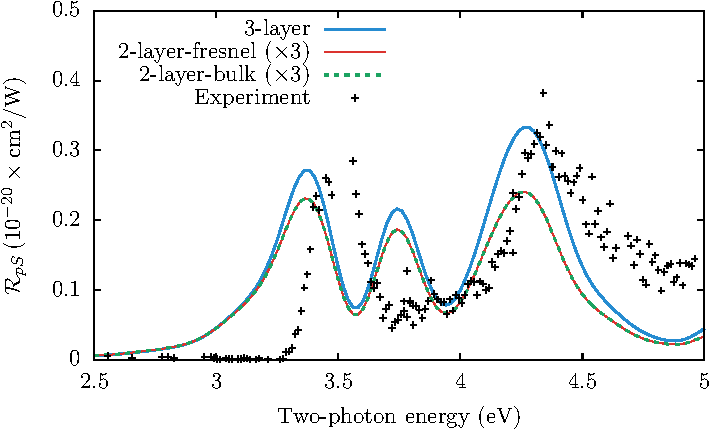
\includegraphics[width=0.7\textwidth]{content/figures/fig-Si1x1-Mejia_RpS}
\caption[$\mathcal{R}_{pS}$ compared to experimental data from Mejia et al.]
{Comparison between theoretical models (see Table \ref{tab:models}) and
experiment for $\mathcal{R}_{pS}$, for $\theta=65^{\circ}$, and a scissors value
of $\hbar\Delta = 0.7\,\text{eV}$. Experimental data taken from Ref.
\cite{mejiaPRB02}, measured at room temperature.}
\label{fig:RpS}
\end{figure}

In Fig. \ref{fig:mitchellRpS}, I compare the theoretical $\mathcal{R}_{pS}$ with
experimental data from Ref. \cite{mitchellSS01}. This calculation uses an angle
of incidence $\theta=45^\circ$ and an azimuthal angle $\phi=30^\circ$ to match
the experimental conditions. As in the previous comparison, the E$_{1}$ peak is
slightly redshifted compared to experiment. The intensity of the theoretical
yield is smaller than the experimental yield for all three models. The
measurements presented in Ref. \cite{mitchellSS01} were taken very shortly after
the surface had been prepared, and the surface itself was prepared with a high
degree of quality and measured at room temperature. Peak position compared to
theory is slightly improved under these conditions. As before, the 3-layer model
is closer in intensity to the experimental spectrum.

\begin{figure}[t]
\centering
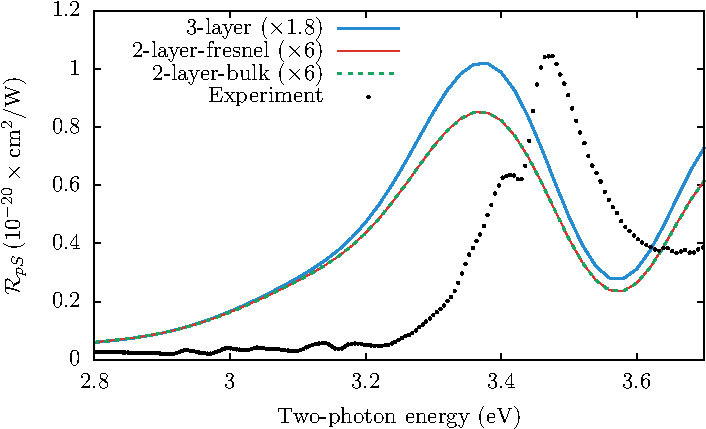
\includegraphics[width=0.7\textwidth]{content/figures/fig-Si1x1-Mitchell_RpS}
\caption[$\mathcal{R}_{pS}$ compared to experimental data from Mitchell et al.]
{Comparison between theoretical models (see Table \ref{tab:models}) and
experiment for $\mathcal{R}_{pS}$, for $\theta=45^\circ$. We use a scissors
value of $\hbar\Delta = 0.7\,\text{eV}$. Experimental data taken from Ref.
\cite{mitchellSS01}, measured at room temperature.}
\label{fig:mitchellRpS}
\end{figure}

From Fig. \ref{fig:Xxxx}, I presented that our calculation for
$\chi^{xxx}_{\mathrm{surface}}$ coincides with the measurement taken at a low
temperature of 80 K. It is well known that temperature causes shifting in the
peak position of SSHG spectra \cite{dadapPRB97}. As $\mathcal{R}_{pS}$ only
depends on this component (see Eq. \eqref{eq:rps111}), the position of the
theoretical peak should be correct in Figs. \ref{fig:RpS} and
\ref{fig:mitchellRpS}. Thus, the difference in peak position should stem from
the higher temperature at which the experiments were measured.

Both the 2-layer-fresnel and 2-layer-bulk models are identical and roughly three
times smaller than the experiment. It is clear from Eq. \eqref{eq:rps111} that
$\mathcal{R}_{pS}$ only has $1\omega$ terms ($\varepsilon_{\ell}(\omega)$ and
$k_{b}$). For both of these models, the fundamental fields are evaluated in the
bulk, which means that the only change to Eq. \eqref{eq:rps111} is that
$\varepsilon_{\ell}(\omega) \rightarrow \varepsilon_{b}(\omega)$. Additionally,
$\Gamma^{\ell}_{pS}$ also remains identical between the two models and has no
$2\omega$ terms in the denominator. Therefore, $r_{pS}$ is identical between
these two models. Ultimately, the intensity of the 3-layer model is the closest
to the experiment. 

Per Eq. \eqref{eq:rps111}, the intensity of $\mathcal{R}_{pS}$ depends only on
$\chi^{xxx}_{\mathrm{surface}}$, which is not affected by local field effects
\cite{tancognedejean:tel-01235611}. These effects are neglected in this
calculation, but $\mathcal{R}_{pS}$ maintains an accurate lineshape and provides
a good quantitative description of the experimental SSHG yield. Note that both
the calculated and experimental spectra show two-photon resonances at the
energies corresponding to the critical point transitions of bulk Si. Note also
that the SSHG yield drops rapidly to zero below E$_{1}$, which is consistent
with the absence of surface states due to the H saturation on the surface. This
observation holds true for all three polarization cases studied for this
surface.

In Fig. \ref{fig:improvements} I provide an overview of the different levels of
approximation proposed in this article. All curves here were calculated using
the 3-layer model. The long dashed line depicts the effect of excluding the
contribution from the nonlocal part of the pseduopotentials. This is consistent
with the results reported in Ref. \cite{andersonPRB15}, where the exclusion of
this term increases the intensity of the components of
$\boldsymbol{\chi}_{\mathrm{surface}}$ by approximately 15\% to 20\%. Note that
the E$_{1}$ peak is larger than the E$_{2}$ peak, contrasting with the
experiment, where the E$_{1}$ peak is smaller than E$_{2}$. The thin solid line
depicts the full calculation with a scissors value of $\hbar\Delta = 0$. The
spectrum is almost rigidly redshifted as this H-saturated surface has no
electronic surface states \cite{andersonPRB15}, in contrast to the
Si(001)(2$\times$1) surface presented in the first part of this chapter. Thus,
this demonstrates the importance of including the scissors correction to
accurately reproduce the experimental spectrum. In summary, the inclusion of the
contribution from the nonlocal part of the pseudopotentials and the scissors
operator on top of the 3-layer model produces spectra with a lineshape and
intensity that compare favorably with the experimental data.

\begin{figure}[t]
\centering
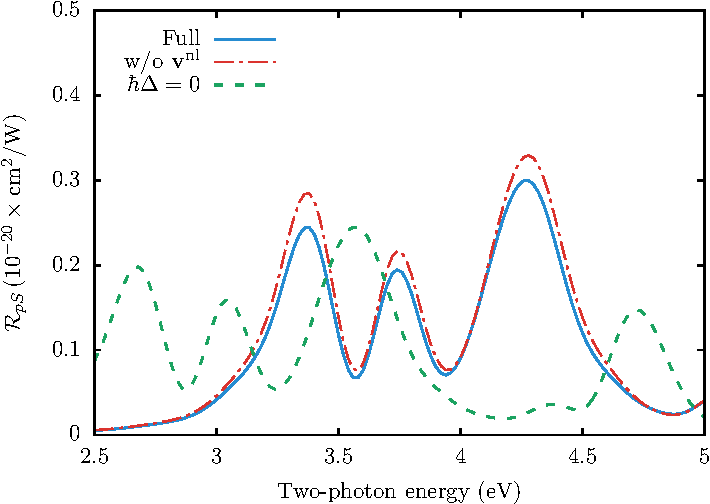
\includegraphics[width=0.7\textwidth]
{content/figures/fig-Si1x1-Mejia_RpS_improvements}
\caption[$\mathcal{R}_{pS}$ calculated with different levels of appoximation.]
{Calculated results for $\mathcal{R}_{pS}$ for the different levels of
approximation proposed in this article. All curves were calculated using the
3-layer model. We take $\theta=65^{\circ}$ for this plot. See text for full
details.}
\label{fig:improvements}
\end{figure}

Lastly, $GW$ transition energies are needed for linear optics and SHG. Doing a
Bethe-Salpeter calculation for SSHG will undoubtedly improve the position and
the amplitude of the peaks, but is far beyond current capabilities \cite{puff}.
I kept the scissors shift constant throughout these calculations as I want to
keep this calculation at the {\em ab initio} level. Remember that the choice of
$\hbar\Delta=0.7$ eV for the scissors shift comes from a $GW$ calculation
\cite{liPRB10}. I have checked that it is not possible to have a single scissors
value that can reproduce the energy positions of both the E$_{1}$ and the
E$_{2}$ peaks. Of course, the experimental temperature at which the spectra is
measured should be taken into account in a more complete formulation. However,
these calculations are always restricted to $T=0$ K. As mentioned before, it is
important to consider the local field effects on the components of
$\chi^{\mathrm{abc}}_{\mathrm{surface}}$. For this surface in particular,
$\chi^{zzz}_{\mathrm{surface}}$ and $\chi^{xxz}_{\mathrm{surface}}$ include
out-of-plane incoming fields. These are affected by local field effects
\cite{tancognedejean:tel-01235611} that reveal the inhomogeneities in the
material, which are much more prevalent perpendicular to the surface than in the
surface plane. This can be evidenced for Si, as Reflectance Anisotropy
Spectroscopy (RAS) measurements are well described by \emph{ab initio}
calculations neglecting local field effects \cite{palummoPRB99, gaalPRB09}. It
is therefore expected that the out-of-plane components will be more sensitive to
the inclusion of local fields. These will not change the transition energies,
only their relative weights of the resonant peaks
\cite{tancognedejean:tel-01235611}. Including these effects is challenging to
compute \cite{nicolasPRB15}, and beyond the scope of this thesis. These effects
would mostly affect $\mathcal{R}_{pP}$ since it includes all four nonzero
components. We speculate that $\mathcal{R}_{pP}$ requires the proper inclusion
of these effects in order to accurately describe the experimental peaks.


%%%%%%%%%%%%%%%%%%%%%%%%%%%%%%%%%%%%%%%%%%%%%%%%%%%%%%%%%%%%%%%%%%%%%%%%%%%%%%%%
%%%%%%%%%%%%%%%%%%%%%%%%%%%%%%%%%%%%%%%%%%%%%%%%%%%%%%%%%%%%%%%%%%%%%%%%%%%%%%%%

\section{Conclusions}

I have used the formulation to calculate the surface nonlinear susceptibility
tensor $\boldsymbol{\chi}_{\mathrm{surface}}$, using the
length gauge formalism and within the independent particle approximation (IPA).
It includes on equal footing: (i) the scissors correction, (ii) the contribution
of the non-local part of the pseudopotentials, and (iii) the cut function. We
have used a Si(001)$2\times 1$ surface to confirm that our scheme correctly
obtains the surface response as we confirm that
$\chi_{\mathrm{half-slab}}^{xxx} \approx
\chi_{\mathrm{full-slab}}^{xxx}$. Although one can in
principle increase the number of atomic layers, $\mathbf{k}$-points, etc. to
improve even further on the similarity of the half-slab and full-slab results,
we have chosen a good compromise between accuracy and the burden and time of the
computations. The effects of the independent inclusion of the three effects
mentioned above in the calculation of
$\boldsymbol{\chi}$ are described as follows. The
scissors correction shifts the spectrum to higher energies though the shifting
is not rigid and mixes the $1\omega$ and $2\omega$ resonances, and has a strong
influence in the line-shape, as for the case of bulk
semiconductors.\cite{luppiJCP10,luppiPRB10,leitsmannPRB05} The cut function
allows us to extract unequivocally $\chi^{xxx}_{2\times
1}$. The effects of the nonlocal part of the
pseudopotentials keeps the same line-shape of $|\chi^{xxx}_{2\times
1}|$, but reduces the value of by 15-20\%. The $xxx$
component of $\boldsymbol{\chi}_{2\times 1}$, can not be
experimentally isolated, however in a forthcoming publication we will compare
our formulation against experimental results. We have neglected local field and
excitonic effects. Although these are important factors in the optical response
of a semiconductor, their efficient calculation is theoretically and numerically
challenging and still under debate \cite{beyond}. This merits further study but
is beyond the scope of this paper. Nevertheless, the inclusion of aforementioned
contributions in our scheme opens the unprecedented possibility to study SSHG
with more versatility and more accurate results.

I also revised the 3-layer model for the SSHG yield where the nonlinear
polarization, $\boldsymbol{\mathcal{P}}(2\omega)$, and the fundamental fields
are taken within a small layer $\ell$ below the surface of the material. This
model reproduces key spectral features and yields an intensity closer to the
experiment for all cases of $\mathcal{R}_{\mathrm{iF}}$. We consider it an
upgrade over the much reviewed 2-layer model\cite{mizrahiJOSA88}, and it comes
with very little added computational expense. Additionally, we have compared
these to other models that change the placement of
$\boldsymbol{\mathcal{P}}(2\omega)$ and the fundamental fields. Ultimately we
consider that the 3-layer model offers the closest comparison to experiment.

This study affords us an interesting view of both the theoretical and
experimental aspects of SSHG studies. On the theoretical side, we have shown the
importance of using relaxed atomic positions to more accurately calculate the
nonlinear susceptibility tensor. The intensity of these spectra is greatly
improved when compared to previous works.\cite{mejiaPRB02} We also postulate
that the lack of local field effects in the theory is a shortcoming, but in this
case, it only affects two of the
$\boldsymbol{\chi}_{\mathrm{surface}}$ components.
Concerning the experiments, we show that surface preparation and quality are
important for better results. The approach for calculating the SSHG yield
presented here finds closer agreement with surfaces that are freshly prepared
with little or no oxidation, and with measurements taken at low temperatures.
Overall, this newly implemented framework for calculating
$\boldsymbol{\chi}_{\mathrm{surface}}$ and $\mathcal{R}$
focused on the Si(001)$2\times 1$ and  Si(111)(1$\times$1):H surfaces provides a
compelling benchmark for SSHG studies. We are confident that this work can be
applied directly to many other surfaces of interest.

\stopcontents[chapters]
